\documentclass[11pt]{report}
\usepackage[utf8]{inputenc}
\usepackage[english]{babel}
\usepackage{hyphenat}
\usepackage{amsmath}
\usepackage{amsfonts}
\usepackage{amssymb}
\usepackage{amsthm}
\usepackage{imakeidx}
\usepackage{hyperref}
\usepackage{enumitem}
\usepackage[boxsize=6pt]{ytableau}
\usepackage{tikz-cd}
\usepackage{tikz}
\usetikzlibrary{decorations.markings,arrows,arrows.meta}
\setlist[enumerate]{itemsep=0mm}
\usepackage[a4paper,left=25mm,right=25mm,top=25mm,bottom=35mm]{geometry}
\linespread{1.275}

\tikzset{every path/.style={thick}}

\newtheorem{theorem}{Theorem}[section]
\newtheorem{lemma}[theorem]{Lemma}
\newtheorem{prop}[theorem]{Proposition}
\newtheorem{corollary}[theorem]{Corollary}
\newtheorem{conjecture}[theorem]{Conjecture}

\theoremstyle{definition}
\newtheorem{definition}[theorem]{Definition}

\theoremstyle{remark}
\newtheorem*{remark}{Remark}

\theoremstyle{remark}
\newtheorem*{example}{Example}

\newenvironment{claim}[1]{\par\noindent\textit{Claim.}\space#1}{}
\newenvironment{claimproof}[1]{\par\noindent\textit{Proof of claim.}\space#1}{\hfill $\Diamond$}

\newcommand{\Diff}{\operatorname{Diff}}
\newcommand{\Hom}{\operatorname{Hom}}
\newcommand{\End}{\operatorname{End}}
\newcommand{\Der}{\operatorname{Der}}
\newcommand{\coim}{\operatorname{coim}}
\newcommand{\im}{\operatorname{im}}
\newcommand{\coker}{\operatorname{coker}}
\newcommand{\id}{\textnormal{id}}
\newcommand{\N}{\mathbb{N}}
\newcommand{\Z}{\mathbb{Z}}
\newcommand{\Q}{\mathbb{Q}}
\newcommand{\R}{\mathbb{R}}
\newcommand{\C}{\mathbb{C}}
\newcommand{\A}{\mathbb{A}}
\newcommand{\F}{\mathbb{F}}
\newcommand{\I}{\mathrm{i}}
\newcommand{\CP}{\mathbb{CP}}
\renewcommand{\P}{\mathbb{P}}

\makeindex[intoc]

\title{
\huge \textsc{~\\~\\ Quantum-classical Duality \\ between Heisenberg and \\ Ruijsenaars-Schneider Models}
}
\author{
-------- \\~\\~\\
Masterarbeit im Masterstudiengang Mathematik \\
der Fakultät für Mathematik, Informatik und Naturwissenschaften \\
der Universität Hamburg \\~\\~\\~\\~\\~\\~\\~\\~\\~\\
}
\date{
\begin{tabular}{ll}
Autor: & Lukas Johannsen \\
Erstgutachter: & Prof. Dr. Gleb Arutyunov \\
Zweitgutachter: & (tba) \\
Ort und Datum: & Hamburg im (tba) 2024
\end{tabular}
}

\begin{document}
\maketitle

~

\thispagestyle{empty}
\setcounter{page}{0}

\pagebreak

\chapter*{Abstract}

We examine a quantum-classical duality between inhomogeneous Heisenberg models and rational Ruijsenaars-Schneider models building on observations of \cite{article:gorsky:2014} and \cite{book:arutyunov:betheAnsatz}. We show how generalized Schur-Weyl duality between the Yangian and the degenerate affine Hecke algebra provides a clear structural reason for the existence of this duality, also giving a generalization to spins in non-fundamental representations. Employing the theory of degenerate double affine Hecke algebras, we extend this point of view to a quantum-classical duality between trigonometric Gaudin and Calogero-Moser models, showing how all four models arise from two $S$-dual representations of the loop Yangian. Finally, we give a geometric picture of generalized Schur-Weyl duality that makes apparent how all of these models emerge naturally in four-dimensional Chern-Simons theory when constructed as a 2-functorial quantum field theory. \\

\section*{Acknowledgments}

I sincerely want to thank my original supervisor Prof. Dr. Gleb Arutyunov for his feedback and guidance in the research process and for sparking my interest in this wonderful topic. He was unfortunately struck with illness during the advising period and I wish him a swift recovery. I also thank (tba) for proofreading the text as well as (tba). Finally, I would like to thank my family for supporting me in my studies.

\tableofcontents

\setcounter{chapter}{-1}
\chapter{Introduction}

Integrability \cite{book:arutyunov:elements} is a key phenomenon in many physical models that allows for exact solutions. Nonetheless, solving integrable models often necessitates surprisingly non-trivial methods. Abstractly, integrability can be understood as the presence of some highly organized structure. Though this can happen in many different ways, a common theme among integrable models is the existence of a large number of commuting conserved quantities. An important tool in discovering such conserved quantities are certain algebras that act on states and observables. Famous representatives in this class of algebras are (double) affine Hecke algebras and affine quantum groups as well as Yangians and their various degenerations, which allow for a reduction of many phenomena in the study of integrable models to phenomena in the representation theory of these algebras. In particular, sharing the same representation theory gives rise to many coincidences in the mathematical descriptions of integrable models, even when these models look very different on the surface. This has led to the discovery of many dualities between integrable models.

In \cite{article:gorsky:2014}, a \emph{quantum-classical} duality between the quantum twisted inhomogeneous Heisenberg $\mathfrak{gl}_\ell$-spin chain and the classical rational Ruijsenaars-Schneider model was first worked out. For our purposes, we will simply refer to this duality as \emph{the} quantum-classical duality. The first model describes a chain of $N$ atoms, labeled by inhomogeneities $y_1,...,y_N \in \C$, whose local Hilbert spaces\footnote{We use the term \emph{Hilbert space} in the loose sense of describing the state space of a quantum system, \emph{i.e.} it does not necessarily come equipped with an inner product. In accordance, we will generally not be careful about Hermiticity.} are given by the vector representation of $\mathfrak{gl}_\ell$. The Hamiltonian imposes nearest-neighbor interactions with boundary conditions that are periodic up to a twist matrix. The second model describes $N$ relativistic point particles acting on each other by mutual centrifugal forces. In this model, the conserved quantities can be neatly described via eigenvalues of a Lax matrix. \emph{Loc. cit.} then describes the quantum-classical duality in terms of a coincidence of spectra of the twist and Lax matrices on the quantum and classical side respectively. This involves the following substitutions: The inhomogeneities of the Heisenberg spin chain model become the positions of the particles in the Ruijsenaars-Schneider model and the eigenvalues of certain non-local spin chain Hamiltonians correspond to the momenta of these particles.

Recently, a novel angle on this duality has appeared in \cite{book:arutyunov:betheAnsatz}, where the Lax matrix of the rational Ruijsenaars-Schneider model miraculously appears in functional relations among higher transfer matrices of the spin chain. Such hints spark the quest for a more conceptual reason behind the coincidence.

To this end, our first step will be to identify the relevant algebras at play. For the Heisenberg $\mathfrak{gl}_\ell$-spin chain, it is well known that its Hilbert space is a representation of the Yangian $Y(\mathfrak{gl}_\ell)$, which in turn contains all relevant observables. For the classical rational Ruijsenaars-Schneider model, it is at first glance more mysterious which algebra we are supposed to consider. However, working with the \emph{quantum} rational Ruijsenaars-Schneider model first, we can identify the degenerate affine Hecke algebra
\begin{equation*}
\dot H_N = \C[S_N] \otimes \C[y_1,...,y_N]
\end{equation*}
contained in the degenerate \emph{double} affine Hecke algebra
\begin{equation*}
\ddot H_N = \C[X_1^{\pm 1},...,X_N^{\pm 1}] \otimes \C[S_N] \otimes \C[y_1,...,y_N],
\end{equation*}
which possesses a representation on $\C[y_1,...,y_N]$ via Macdonald difference operators that yields the relevant wave functions, \emph{i.e.} the generators $y_i$ become the position operators of the particles and the generators $X_i$ correspond to momentum operators. We will show how the coincidence in the descriptions of the Heisenberg and Ruijsenaars-Schneider models can be summarized by twisting an old result of Drinfeld \cite{article:drinfeld:1986}: There exists a generalized Schur-Weyl functor from the category of $\dot H_N$-modules to the category of $Y(\mathfrak{gl}_\ell)$-modules, which is fully faithful when $\ell > N$, giving an equivalence between $\dot H_N$-modules and $Y(\mathfrak{gl}_\ell)$ of weight $N$. Applying this functor to the wave function representation $\C[y_1,...,y_N]$ reduces to the sought-after result, yielding the representation
\begin{equation*}
(\C^\ell)^{\otimes N} \otimes_{S_N} \C[y_1,...,y_N]
\end{equation*}
of the Yangian, on which the momentum-like operators $X_i$ act exactly as the non-local Hamiltonians of the spin chain when the Planck constant $\hbar$ of the rational Ruijsenaars-Schneider model goes to zero.

This is however not the full picture. The fact that we are suddenly dealing with the Laurent generators $X_i$ from the degenerate \emph{double} affine Hecke algebra points to a missing piece. Recall that \emph{non}-degenerate double affine Hecke algebras have an $S$-duality automorphism by way of interchanging their two sets of Laurent generators. As a remnant of this $S$-duality, the representation of $\ddot H_N$ on $\C[y_1,...,y_N]$ above has an $S$-dual representation on $\C[X_1^{\pm 1},...,X_N^{\pm 1}]$ via Dunkl differential operators. This representation describes the quantum trigonometric Calogero-Moser model. In a similar fashion as above, we can view it as a representation of the affine symmetric group $\dot S_N = S_N \ltimes \Z^N$ which sits inside $\ddot H_N$. Using Schur-Weyl duality for affine symmetric groups, we obtain a representation of the loop algebra $L(\mathfrak{gl}_\ell)$. We then combine the action of the loop algebra and the action of the Yangian to an action of the loop Yangian $LY(\mathfrak{gl}_\ell)$, unifying all four models using generalized Schur-Weyl duality between the degenerate double affine Hecke algebra and the loop Yangian \cite{article:guay:2005}.%, to unify all four models: The rational Ruijsenaars-Schneider model, the Heisenberg model, the trigonometric Calogero-Moser model, and the trigonometric Gaudin model all arise as representations of the loop Yangian.

To finish our discussion, we will reframe this representation theoretic picture in a more geometric setting, thus connecting it to gauge theory. It will turn out that the whole story can be retold in terms of four-dimensional Chern-Simons theory, which was first described in \cite{article:costello:2013} and subsequently expanded on in a series of papers starting with \cite{article:costello:2018}. Four-dimensional Chern-Simons theory is a semi-topological quantum field theory or, more precisely, holomorphic in two directions with complex coordinate $z$ and topological in the other two directions. Thus, it lives on a four-manifold $C \times \Sigma$, where $C$ is a complex curve and $\Sigma$ an oriented surface. Its main dynamical variable is a $\mathfrak{gl}_\ell$-valued connection 1-form $A(z)$ on $\Sigma$, which is meromorphic in $z \in C$. One also fixes a meromorphic 1-form $\omega$ on $C$, which is wedged with the Chern-Simons 3-form of $A$ to obtain the Langrangian density of the theory. Its poles and zeros respectively give rise to order and disorder defects of the gauge field $A$.

\begin{figure}
\begin{tikzpicture}[remember picture,overlay]
  \node[opacity=0.1] at (7.45cm,-4.9cm) {
    
\includegraphics[width=11cm, height=7.5cm]{src/butterfly}
  };
\end{tikzpicture}
\begin{center}
\begin{tikzcd}[column sep=0.5cm,row sep=1.5cm]
\text{Heisenberg model} \arrow[leftrightarrow,bend right=50]{dd} \arrow[leftrightarrow,bend left=40]{rr} & & \text{Gaudin model} \arrow[leftrightarrow,bend left=50]{dd} \\
\C \times S^1 \times \R & \arrow[bend left=20]{ul} \arrow[bend right=20]{dl} \text{4d CS} \arrow[bend right=20]{ur} \arrow[bend left=20]{dr} & \C^\times \times \R^2 \\
\text{rational RS model} \arrow[leftrightarrow,bend right=40]{rr} & & \text{trigonometric CM model}
\end{tikzcd}
~\\~\\
\end{center}
\caption{A pictorial summary of the results. The reflection symmetry around the horizontal axis comes from generalized Schur-Weyl duality, while the reflection symmetry around the horizontal axis comes from $S$-duality. Here we respectively write $\CP^1$ without the double pole at infinity as $\C$ and $\CP^1$ without the single poles at zero and infinity as $\C^\times$.}
\label{figure:dualities}
\end{figure}

Specializing four-dimensional Chern-Simons theory to the four-manifold $C \times \Sigma$ with $C = \CP^1$ and the 1-form
\begin{equation*}
\omega = \frac{(z-y_1-\eta) \cdots (z-y_N-\eta)}{(z-y_1) \cdots (z-y_N)} dz,
\end{equation*}
where $\eta$ is the Planck constant of the theory, as well as $\Sigma = S^1 \times \R$ a cylinder, we will see how the rational Ruijsenaars-Schneider model describes the boundary conditions at the order defects $y_i$ of the gauge field $A$ while Wilson loops around the cylinder describe the transfer matrices of the Heisenberg model. $S$-Dually, we may also specialize to $C = \CP^1$ with
\begin{equation*}
\omega = (?) \frac{dz}{z}
\end{equation*}
and $\Sigma = \R^2$. (tba) The entire situation is summarized by the mock commutative diagram in figure \ref{figure:dualities}.

The remaining chapters of this thesis are structured as follows. Chapter \ref{chapter:integrability} gives a full review from the basics of integrability to the state of the art of the pertinent models and establishes the setup that frames our discussion. Chapter \ref{chapter:duality} begins with a detailed discussion of the recent appearance of the Lax matrix of the Ruijsenaars-Schneider model in the functional relations for transfer matrices of the Heisenberg model used to derive the spectral equation whose solutions yield the energy spectrum of the Heisenberg model. We then move on to describe the mathematical underpinnings of generalized Schur-Weyl duality and how it gives rise to quantum-classical duality. The end of chapter \ref{chapter:duality} is dedicated to explicating $S$-duality, showing how the $S$-dual models, \emph{i.e.} the trigonometric Gaudin model and the trigonometric Calogero-Moser model are also related by quantum-classical duality. Chapter \ref{chapter:geometry} then continues with a description of the geometry behind the mathematical structures of chapter \ref{chapter:duality}, constructing two functorial field theories: One encapsulating Heisenberg-Ruijsenaars-Schneider duality and the other $S$-dual theory encapsulating Gaudin-Calogero-Moser duality. Each are shown to arise from four-dimensional Chern-Simons theory. After the conclusion (chapter \ref{chapter:conclusion}), we give supplementary material on Young diagrams (appendix \ref{appendix:youngdiagrams}) as well as results on Dunkl operators for the trigonometric Calogero-Moser model (appendix \ref{appendix:dunklOperators}).

~\\

\begin{center}
\textit{-- Enjoy! --}
\end{center}

%%%%%%%%%%%%%%%%%%%%%%%%%%%%%%%%%%%%%%%%%

\chapter{Integrability}\label{chapter:integrability}

\section{Classical integrability}

\subsection{Liouville theorem}

Physical models in classical mechanics are described by phase spaces that are $2N$-dimensional symplectic manifolds together with a choice of Hamiltonian $H$. In this setting, the definitive definition of integrability is given by \emph{Liouville integrability}, which comes from the basic idea that conserved quantities reduce the effective dimensionality of the phase space. To see this, assume that we are handed a conserved quantity $f$, in other words $\dot f = \{ H, f \} = 0$. By definition, $f$ will be constant along the Hamiltonian flow generated by the Hamiltonian vector field of $H$, say $f \equiv c \in \R$, so we may narrow our phase space to individual level sets of $f$, which generically have codimension one. Continuing this argument inductively by adding more conserved quantities while making sure that they all Poisson-commute, one will eventually arrive at a half-dimensional submanifold on which the equations of motion simplify greatly. This requires a full set of $N$ independent Poisson-commuting observables, including the Hamiltonian:

\begin{theorem}[Liouville theorem \cite{book:arnold}] \index{Liouville theorem}
Let $M$ be a $2N$-dimensional symplectic manifold and suppose there exist $N$ smooth functions $f_1,...,f_N \in C^\infty(M)$ such that all pairwise Poisson brackets vanish, \emph{i.e.} $\{ f_i,f_j \} = 0$ for all $1 \leq i,j \leq N$ and the Hamiltonian $H$ is a function of the $f_i$. Given $c = (c_1,...,c_N) \in \R^N$, consider the level set
\begin{equation*}
M_c := \{ p \in M \mid f_i(p) = c_i \}.
\end{equation*}
If the 1-forms $df_i$ are linearly independent on $M_c$, then:
\begin{enumerate}[label=(\roman*)]
\item $M_c$ is a smooth submanifold invariant under the Hamiltonian flow.
\item If $M_c$ is compact and connected, then $M_c$ is diffeomorphic to $(S^1)^N$. In this case, the Hamiltonian flow for $H$ is linearly periodic, \emph{i.e.}
\begin{equation*}
\dot \varphi_i = \omega_i
\end{equation*}
for $\varphi_i$ the $i$th angular coordinate and $\omega_i$ a frequency dependent only on $c$ and $H$.
\end{enumerate}
\end{theorem}

\begin{proof}
tba
\end{proof}

\begin{example}
The simplest example of a Liouville integrable model is the classical harmonic oscillator. Its phase space is $(\R^2,dp \wedge dq)$ with Hamiltonian
\begin{equation*}
H(p,q) = \tfrac{1}{2} (p^2 + q^2).
\end{equation*}
The Hamiltonian itself trivially provides enough conserved quantities for Liouville integrability to hold. This directly manifests in the time evolution of the harmonic oscillator: For a fixed energy $E = \frac{\alpha^2}{2}$, the equations of motion reduce to $\dot \varphi = 1$, where we have introduced the angular variable $\varphi$ parameterizing $p$ and $q$ via
\begin{equation*}
p(\varphi) = \alpha \cos(\varphi), \quad q(\varphi) = \alpha \sin(\varphi).
\end{equation*}
This is easily generalized to $N$ uncoupled, possibly anisotropic harmonic oscillators with phase space $(\R^{2N},\sum_i dp_i \wedge dq_i)$, conserved quantities
\begin{equation*}
f_i = \tfrac{1}{2}(p_i^2 + \omega_i^2 q_i^2), \quad \omega_i \in \R,
\end{equation*}
and Hamiltonian $H = \sum_i f_i$. The level sets for these integrals of motion are of the form $(S^1)^N$ with angular variables $\varphi_1,...,\varphi_N$ evolving linearly as $\dot \varphi_i = \omega_i$. Note that the time evolution is only truly periodic when the $\omega_1,...,\omega_N$ are all integer multiples of a fundamental frequency.
\end{example}

\subsection{Lax pairs}

The Liouville theorem leaves open the following question: How do we find enough conserved quantities? This is generally a very hard task, but there are some structures that can help us. One important such structure is the existence of a \emph{Lax pair}:

\begin{definition} \index{Lax pair}
A pair $(L,M)$ of $n \times n$ matrices of observables is a \emph{Lax pair} if the \emph{Lax equation}
\begin{equation*}
\dot L = [M,L].
\end{equation*}
holds. We then call $L$ a \emph{Lax matrix}.
\end{definition}

\begin{remark}
Lax pairs are not unique. In fact, any Lax pair may be twisted by an invertible matrix of observables $g$ via the gauge-like transformation
\begin{equation*}
L \mapsto gLg^{-1}, \quad M \mapsto gMg^{-1} + \dot g g^{-1}
\end{equation*}
We may also add any polynomial in $L$ to $M$ without changing the Lax equation.
\end{remark}

\begin{prop}
Given a Lax pair $(L,M)$, the spectral invariants $I_k := \operatorname{tr} L^k$ for $k \in \Z$ constitute a family of conserved quantities.
\end{prop}

\begin{proof}
Notice that $L^{-1}$ is also a Lax matrix:
\begin{equation*}
\dot L^{-1} = - L^{-1} \dot L L^{-1} = -L^{-1} [M,L] L^{-1} = [M,L^{-1}].
\end{equation*}
Hence, for $k \geq 0$ we obtain
\begin{equation*}
\dot I_{\pm k} = k \operatorname{tr} (L^{\pm 1})^{k-1} \dot L^{\pm 1} = k \operatorname{tr} (L^{\pm 1})^{k-1} [M,L^{\pm 1}] = k \operatorname{tr} [M,L^{\pm k}] = 0,
\end{equation*}
making use of the cyclic property of the trace.
\end{proof}

\begin{example}
Let us again consider the harmonic oscillator and introduce the matrices
\begin{equation*}
L = \frac{1}{2}
\begin{pmatrix}
p & q \\ q & -p
\end{pmatrix},
\quad
M = \frac{1}{2}
\begin{pmatrix}
0 & -1 \\
1 & 0
\end{pmatrix}
\end{equation*}
We check
\begin{equation*}
\dot L = \frac{1}{2}
\begin{pmatrix}
-q & p \\ p & q
\end{pmatrix}
=
\frac{1}{4}
\begin{pmatrix}
p & q \\ q & -p
\end{pmatrix}
\begin{pmatrix}
0 & -1 \\
1 & 0
\end{pmatrix}
-
\frac{1}{4}
\begin{pmatrix}
0 & -1 \\
1 & 0
\end{pmatrix}
\begin{pmatrix}
p & q \\ q & -p
\end{pmatrix}
= [M,L]
\end{equation*}
and see that the conserved quantity $\operatorname{tr} L^2 = \frac{1}{2}(p^2+q^2)$ is the Hamiltonian.
\end{example}

We quickly remark that the existence of a Lax pair is by itself insufficient to guarantee Liouville integrability. Firstly, it might fail to produce enough \emph{independent} conserved quantities, and secondly, it might fail to produce \emph{Poisson-commuting} conserved quantities. However, there is a way to guarantee that the spectral invariants of the Lax matrix Poisson-commute. We briefly state this result here:

\begin{theorem}[Babelon-Viallet \cite{book:arutyunov:elements}]
The eigenvalues of a matrix $L$ of observables on a phase space $(M,\omega)$ Poisson-commute if and only if there exists a so-called \emph{dynamical $r$-matrix}
\begin{equation*}
r \in \operatorname{Mat}_n(C^\infty(M))^{\otimes 2}
\end{equation*}
with
\begin{equation*}
\{ L_1, L_2 \} = [r_{12},L_1] - [r_{21},L_2],
\end{equation*}
where $L_1,L_2$ respectively denote $L \otimes 1, 1 \otimes L$ and $r_{21},r_{12}$ respectively denote $r$ with and without the tensor factors swapped.
\end{theorem}

\subsection{Lax connections}

The definition of a Lax pair arguably looks ad hoc. One way to see how this structure makes sense is to look at how Lax pairs arise from the flatness equation of so called \emph{Lax connections} in two-dimensional field theories. For later purposes, we will consider Lax connections with a \emph{spectral parameter}.

\begin{definition}
Let $\Sigma$ be an oriented surface and $\mathfrak{g}$ a semi-simple Lie algebra. A \emph{Lax connection with spectral parameter}\index{Lax connection}\index{Spectral parameter} is a $\mathfrak{g}$-valued 1-form $A(z)$ on $\Sigma$ meromorphic in $z$ such that $A(z)$ is flat when $z$ is not a pole. Writing
\begin{equation*}
A(z) = A_t(z) dt + A_x(z) dx
\end{equation*}
in local coordinates $t,x$, this means
\begin{equation*}
\partial_t A_x(z) - \partial_x A_t(z) = [A_t(z),A_x(z)].
\end{equation*}
\end{definition}

\begin{prop}
Let $\Sigma = \R \times S^1$ be a cylinder with axial coordinate $t$ and angular coordinate $x$ and $A = A_t dt + A_x dx$ be a Lax connection. Let $z$ not be a pole and
\begin{equation*}
L(z) := \operatorname{Hol}_\gamma(A), \quad M(z) := A_t(z)|_{x=0},
\end{equation*}
where $\gamma$ is a loop winding once around the cylinder and $\operatorname{Hol}_{\gamma_t}(A)$ denotes the holonomy of $A$ around $\gamma$, which is invariant under homotopies due to flatness. Then $(L(z),M(z))$ is a Lax pair.
\end{prop}

\begin{proof}
Let $\gamma$ be a curve starting at $(t_0,x_0) \in \Sigma$ and ending at $(t_1,x_1) \in \Sigma$. The defining partial differential equations for the holonomy give
\begin{equation*}
\frac{\partial}{\partial t_0} \operatorname{Hol}_\gamma(A) = -A_t(z)|_{x=x_0} \operatorname{Hol}_\gamma(A), \quad \frac{\partial}{\partial t_1} \operatorname{Hol}_\gamma(A) = A_t(z)|_{x=x_1} \operatorname{Hol}_\gamma(A).
\end{equation*}
Choosing $x_0 = x_1 = 0$ and letting $\gamma$ wind once around the cylinder implies
\begin{equation*}
\dot L(z) = \frac{\partial}{\partial t_0} \operatorname{Hol}_\gamma(A) + \frac{\partial}{\partial t_1} \operatorname{Hol}_\gamma(A) = A_t(z)|_{x=0} \operatorname{Hol}_\gamma(A) - A_t(z)|_{x=0} \operatorname{Hol}_\gamma(A) = [M(z),L(z)],
\end{equation*}
which shows that we indeed have a Lax pair.
\end{proof}

\begin{remark}
The conserved quantities $I_k(z) = \operatorname{tr} L(z)^k$ arising from Lax connections on a cylinder $\Sigma = \R \times S^1$ are exactly the traces of holonomies of loops with winding number $k$ around the cylinder. We may expand $I_k(z)$ around $z=0$ to obtain an infinite tower of conserved quantities.
\end{remark}

\subsection{Ruijsenaars-Schneider and Calogero-Moser models}

We now come to two very important classes of examples of classical integrable models: The Ruijsenaars-Schneider and Calogero-Moser models.

\begin{definition}
The \emph{classical Ruijsenaars-Schneider models}\index{Ruijsenaars-Schneider model}, originally constructed in \cite{article:ruijsenaars:1987}, for $N$ particles of positions $y_i$ and momenta $p_i$, speed of light $c$, and coupling constant $\eta$ have the Hamiltonians
\begin{equation}\label{equation:ratRSHamiltonian}
H^\text{RS} := \sum_i \cosh(p_i/c) \prod_{i \neq j} \sqrt{1 + \frac{u(y_i - y_j)}{u(\eta/c)}}
\end{equation}
with $u(y) := 1/y^2$ for the rational and $u(y) := 1/(4\sinh^2(y/2))$ for the trigonometric case.
\end{definition}

For the sequel, we will set $c=1$, though we first note that setting
\begin{equation}\label{equation:trigCMHamiltonian}
H^\text{CM} := \frac{1}{2} \sum_i p_i^2 + \frac{\eta^2}{2} \sum_{i \neq j} u(y_i-y_j),
\end{equation}
and expanding $H^\text{RS}$ around $c = \infty$ yields

\begin{prop}
\begin{equation*}
H^\textnormal{RS} = N + \bigg( \frac{1}{c} \bigg)^2 H^\textnormal{CM} + \mathcal{O}\bigg( \bigg( \frac{1}{c} \bigg)^4 \bigg).
\end{equation*}
\end{prop}

\begin{proof}
This is a quick computation with Mathematica ($\to$ \texttt{RSHamiltonianExpansion.nb}).
\end{proof}

\begin{definition}
The function $H_\text{CM}$ from equation (\ref{equation:trigCMHamiltonian}) defines the Hamiltonians for the \emph{classical Calogero-Moser models}\index{Calogero-Moser model}.
\end{definition}

The Hamiltonian (\ref{equation:trigCMHamiltonian}) of the rational Calogero-Moser model evidently describes point particles repelling each other through centrifugal inverse-cube forces. \cite{article:ruijsenaars:1987} hence argues that the rational Ruijsenaars-Schneider model describes the same phenomenon in the relativistic setting with finite speed of light $c$. The trigonometric case might be thought of as a periodic modification after taking the position variables $y_i$ to be purely imaginary, hence describing particles on a circle. Our focus will be on the rational Ruijsenaars-Schneider model and the trigonometric Calogero-Moser model.

\begin{prop}
Lax matrices ensuring Liouville integrability for the rational Ruijsenaars-Schneider and the trigonometric Calogero-Moser model are given by
\begin{equation}\label{equation:RSLaxMatrix}
L_{ij}^\textnormal{RS} = \frac{\eta}{y_i-y_j+\eta} \bigg( \prod_{k \neq j} \frac{y_j-y_k-\eta}{y_j-y_k} \bigg) e^{-p_j}
\end{equation}
and
\begin{equation*}
L_{ij}^\textnormal{CM} = \delta_{ij} p_i + (1-\delta_{ij}) \eta \theta_{ij}, \quad \theta_{ij} := \frac{e^{y_i}}{e^{y_i}-e^{y_j}}.
\end{equation*}
\end{prop}

\begin{proof}
See \cite{book:arutyunov:elements}.
\end{proof}

\begin{remark}
For the rational Ruijsenaars-Schneider model, we will make use of the alternative Hamiltonian
\begin{equation}\label{equation:ratRSHamiltonianPrime}
\operatorname{tr} L^\textnormal{RS} = \sum_i \bigg( \prod_{i \neq j} \frac{y_i-y_j-\eta}{y_i-y_j} \bigg) e^{-p_i}.
\end{equation}
Choosing this Hamiltonian is mostly a matter of convention, as $\operatorname{tr} L^\textnormal{RS} + \operatorname{tr}(L^\textnormal{RS})^{-1}$ is equivalent to (\ref{equation:ratRSHamiltonian}) up to a canonical transformation \cite{book:arutyunov:elements}. Note that for the trigonometric Calogero-Moser model we already have
\begin{equation*}
\tfrac{1}{2} \operatorname{tr} (L^\textnormal{CM})^2 = H^\textnormal{CM}
\end{equation*}
due to $\theta_{ij} \theta_{ji} = 1/(4 \sinh^2((y_i-y_j)/2))$.
\end{remark}

\section{Quantum integrability}

Integrability in the quantum context is generally considered to be a more diffuse concept than classical integrability. The basic definition generalizing Liouville integrability is the existence of a large set of mutually commuting quantum observables that include the Hamiltonian. Such can often be guaranteed by the existence of operators fulfilling the quantum Yang-Baxter equation or the applicability of various Bethe ansätze \cite{book:arutyunov:betheAnsatz}. This usually comes hand-in-hand with the existence of large symmetries, especially \emph{Hecke symmetries} and \emph{Yangian symmetries}, which automatically generate sets of commuting operators via their commutative subalgebras.

In order to quantize the rational Ruijsenaars-Schneider and trigonometric Calogero-Moser model, we will start with a discussion of Hecke algebras and their representations, after which we move on to the Yangian of $\mathfrak{gl}_\ell$, whose representation theory gives rise to the Heisenberg model.

\subsection{Weyl groups and Hecke algebras of type $A$}

Let $N$ be a natural number. The Weyl group of type $A_{N-1}$ is the symmetric group $S_N$ on $N$ letters. We write cycles in standard form $(1 \ 2 \ 3)$, mapping 1 to 2, 2 to 3, and 3 to 1, and denote the simple transpositions $(i \ i+1)$ by $s_i$ for $1 \leq i < N$. Finally, we let $w := s_1 \cdots s_{N-1}$ denote the Coxeter element.

\begin{definition}
\begin{enumerate}[label=(\roman*)]
\item The \emph{affine Weyl group of type $A_{N-1}$} is the group $\dot S_N := S_N \ltimes \Z^N$, where $S_N$ acts on $\Z^N$ by permutation of coordinates. The group algebra $\C[\dot S_N]$ is canonically generated by the group algebra $\C[S_N]$ of the symmetric group and an algebra of Laurent polynomials $\C[X_1^{\pm 1},...,X_N^{\pm 1}]$. In fact, it is generated by the simple transpositions $s_i$ and the element $\pi := X_1 w$.
\item The \emph{degenerate double affine Hecke algebra (of type $A_{N-1}$)}\index{Degenerate double affine Hecke algebra} is the $\C[\eta,\hbar]$-algebra $\ddot H_N$ generated by the group algebra $\C[\dot S_N]$ and the polynomial algebra $\C[y_1,...,y_N]$ subject to the cross-relations
\begin{align*}
s_i y_j = y_j s_i, \quad s_i y_i = y_{i+1} s_i + \eta, \quad \pi y_i \pi^{-1} = y_{i+1}, \quad \pi y_N \pi^{-1} = y_1 + \I \hbar,
\end{align*}
where $1 \leq i < N, 1 \leq j \leq N$ and $|i-j|>1$. It can thus be seen to be generated by the simple transpositions $s_i$ as well as $\pi$ and $y_1$. Let us also remark that these relations admit an anti-automorphism
\begin{equation*}
s_i \mapsto s_i, \quad X_i \mapsto X_i^{-1}, \quad y_i \mapsto y_i,
\end{equation*}
making left modules equivalent to right modules.
\item The $\C[\eta]$-subalgebra $\dot H_N \subset \ddot H_N$ generated only by $\C[S_N]$ and $\C[y_1,...,y_N]$ is the \emph{degenerate affine Hecke algebra (of type $A_{N-1}$)}\index{Degenerate affine Hecke algebra}. It is also generated by the $s_i$ and $y_1$.
\item Let $e := \frac{1}{N!}\sum_{\sigma \in S_N} \sigma \in \ddot H_N$ be the symmetrizer. Then $S\ddot H_N := e \ddot H_N e$ is the \emph{spherical degenerate double affine Hecke algebra (of type $A_{N-1}$)}\index{Spherical degenerate double affine Hecke algebra}.
\end{enumerate}
\end{definition}

The spherical degenerate double affine Hecke algebra will be of great importance, since it produces families of commuting operators by the following proposition: 

\begin{prop}
\begin{enumerate}[label=(\roman*)]
\item $S\ddot H_N$ is finitely generated and commutative.
\item The degenerate double affine Hecke algebra $\ddot H_N$ is finite over $S\ddot H_N$.
\item Specializing to $\hbar = 0$, there is the Satake isomorphism $Z(\ddot H_N) \overset \sim \to S\ddot H_N, z \mapsto ze$, while one has $Z(\ddot H_N) = \C$ for $\hbar \neq 0$.
\item The spectrum of $S\ddot H_N$ is the configuration space of the classical rational Ruijsenaars-Schneider and trigonometric Calogero-Moser model.
\end{enumerate}
\end{prop}

\begin{proof}
See \cite{article:oblomkov:2003}.
\end{proof}

Much of the following is in analogy to \cite{article:lamers:2022}, where the non-degenerate case is discussed. We construct a representation of $\dot H_N$ on polynomials $\C[y_1,...,y_N]$. Let us begin by considering the action where $S_N$ acts by permutation of the variables. This allows us to introduce the following operators:
\begin{enumerate}[label=(\roman*)]
\item The \emph{divided difference operators} are defined as
\begin{equation*}
\Delta_i := (y_i-y_{i+1})^{-1} (1-s_i).
\end{equation*}
Note that the anti-symmetrization implies that $\Delta_i^2 = 0$ and that $\Delta_i f$ for any polynomial $f$ will again be a polynomial despite its denominator. We further note that $\Delta_i y_i = y_{i+1} \Delta_i + 1$.
\item The \emph{$T$-operators} are defined as
\begin{equation*}
T_i := s_i + \eta \Delta_i = \frac{y_i-y_{i+1}-\eta}{y_i-y_{i+1}} s_i + \frac{\eta}{y_i-y_{i+1}}.
\end{equation*}
\end{enumerate}

\begin{lemma}
The mapping
\begin{align*}
s_i \mapsto T_i, \quad y_i \mapsto y_i
\end{align*}
gives rise to a representation of $\dot H_N$ on $\C[y_1,...,y_N]$.
\end{lemma}

\begin{proof}
It is clear that $T_i$ and $T_j,y_j$ commute for $|i-j|>1$. We also have
\begin{equation*}
T_i^2 = 1 + s_i \eta \Delta_i + \eta \Delta_i s_i = 1 + \eta \Delta_i - \eta \Delta_i = 1.
\end{equation*}
as well as the braid relation $T_i T_{i-1} T_i = T_{i-1} T_i T_{i-1}$, which may be quickly checked in Mathematica ($\to$ \texttt{TOperatorRelations.nb}). The relation $T_i y_i = y_{i+1} T_i + \eta$ follows readily from $\Delta_i y_i = y_{i+1} \Delta_i + 1$.
\end{proof}

\begin{prop}
Let $\pi$ act on $\C[y_1,...,y_N]$ by
\begin{equation*}
(\pi f)(y_1,...,y_N) := f(y_2,...,y_N,y_1 + \I \hbar).
\end{equation*}
The mapping
\begin{align*}
s_i \mapsto T_i, \quad X_i \mapsto T_{i-1} \cdots T_1 \pi T_{N-1} \cdots T_i, \quad y_i \mapsto y_i
\end{align*}
gives rise to a representation of $\ddot H_N$ on $\C[y_1,...,y_N]$.
\end{prop}

\begin{proof}
It is clear that the action of $\pi$ fulfills the necessary relations between $\pi$ and the $y_i$. Furthermore, we see that $X_1 = \pi w^{-1}$ acts as $\pi T_{N-1} \cdots T_1$, from which the general form for $X_i$ follows.
\end{proof}

There is an obvious representation of $\dot S_N$ on Laurent polynomials $\C[X_1^{\pm 1},...,X_N^{\pm 1}]$ where $S_N$ permutes the variables and $X_i$ acts simply by multiplication. This representation also extends to $\ddot H_N$ in the following way:

\begin{prop}\label{prop:trigCMRepresentation}
Let $\theta_{ij} := X_i/(X_i-X_j)$. The mapping
\begin{align*}
s_i \mapsto s_i, \quad X_i \mapsto X_i, \quad y_i \mapsto -\I \hbar X_i \partial_i - i \eta + \eta \sum_{j < i} \theta_{ji} (1-(i \ j)) - \eta \sum_{j > i} \theta_{ij} (1-(i \ j))
\end{align*}
gives rise to a representation of $\ddot H_N$ on $\C[X_1^{\pm 1},...,X_N^{\pm 1}]$.
\end{prop}

\begin{proof}
We refer to appendix \ref{appendix:dunklOperators}, lemma \ref{lemma:trigCMRepresentationAppendix}.
\end{proof}

\begin{remark}
The operators $X_i$ acting on $\C[y_1,...,y_N]$ are called \emph{Macdonald operators}, while the operators $y_i$ acting on $\C[X_1^{\pm 1},...,X_N^{\pm 1}]$ are called \emph{Dunkl operators}.
\end{remark}

\subsection{Quantization of Ruijsenaars-Schneider and Calogero-Moser models}

We will now show that the former polynomial representation above yields the rational Ruijsenaars-Schneider model, while the latter yields the trigonometric Calogero-Moser model. More precisely, we will see that certain symmetric polynomials in the $X_i$ and $y_i$ respectively yield the correct Hamiltonians. This manifests the bispectral duality between those two systems \cite{article:chalykh:2000} as a remnant of the $S$-duality exchanging the two sets of Laurent generators of the non-degenerate double affine Hecke algebra.

\begin{definition}
The \emph{quantum rational Ruijsenaars-Schneider model} is essentially given by the former polynomial representation of the degenerate double affine Hecke algebra\index{Quantum rational Ruijsenaars-Schneider model}. Concretely, its Hilbert space of wave functions is nothing but the vector space $\C[y_1,...,y_N]$, where the polynomial generators $y_1,...,y_N$ provide position operators while the Laurent generators $X_1,...,X_N$ provide operators involving momenta. Of particular interest is the spherical subalgebra $S\ddot H_N$, from which we get commuting Hamiltonians
\begin{equation*}
D_k := e_k(X_1,...,X_N) \in S\ddot H_N,
\end{equation*}
with $e_k$ the $k$th elementary symmetric polynomial.
\end{definition}

\begin{lemma}
Let
\begin{equation*}
x_{ji} := \frac{y_i-y_j-\eta}{y_i-y_j} + \frac{\eta}{y_i-y_j} (i \ j).
\end{equation*}
Then
\begin{equation*}
X_i = x_{i,i-1} \cdots x_{i1} e^{\I \hbar \partial_i} x_{iN} \cdots x_{i,i+1}.
\end{equation*}
when acting on $\C[y_1,...,y_N]$.
\end{lemma}

\begin{proof}
Observe that $T_i s_i = x_{i+1,i}$ and $s_i T_i = x_{i,i+1}$, hence
\begin{align*}
T_{i-1} \cdots T_1 \pi T_{N-1} \cdots T_i
&= T_{i-1} \cdots T_1 e^{\I \hbar \partial_1} s_1 \cdots s_{N-1} T_{N-1} \cdots T_i \\
&= T_{i-1} \cdots T_1 s_1 \cdots s_{i-1} e^{\I \hbar \partial_i} s_i \cdots s_{N-1} T_{N-1} \cdots T_i \\
&= x_{i,i-1} \cdots x_{i1} e^{\I \hbar \partial_i} x_{iN} \cdots x_{i,i+1}.
\end{align*}
\end{proof}

\begin{prop}
On symmetric polynomials, \emph{i.e.} bosonic wave functions, $D_1$ reduces to the canonically quantized Hamiltonian (\ref{equation:ratRSHamiltonianPrime}) of the rational Ruijsenaars-Schneider model:
\begin{equation*}
D_1 = \sum_i \bigg( \prod_{i \neq j} \frac{y_i-y_j-\eta}{y_i-y_j} \bigg) e^{\I \hbar \partial_i}.
\end{equation*}
\end{prop}

\begin{proof}
We proceed in analogy to \cite{article:jimbo:1995}. We know that $X_i$ acts as
\begin{equation*}
x_{i,i-1} \cdots x_{i1} e^{\I \hbar \partial_i} x_{iN} \cdots x_{i,i+1}
\end{equation*}
by the previous lemma. It is clear that $x_{ij}$ acts as the identity on symmetric polynomials. Note however that while $D_1$ does preserve the space of symmetric polynomials, $e^{\I \hbar \partial_i}$ on its own does not, so the $x_{ij}$ to the left of $e^{\I \hbar \partial_i}$ act non-trivially. Pulling the permutations to the right yields
\begin{equation*}
\bigg( \prod_{j < i} \frac{y_i-y_j-\eta}{y_i-y_j} \bigg) e^{\I \hbar \partial_i} + (\text{terms for } e^{\I \hbar \partial_j} \text{ with } j < i).
\end{equation*}
In particular, we see that only $X_N$ contributes to the coefficient in front of $e^{\I \hbar \partial_N}$, which is exactly $\prod_{N \neq j} \frac{y_N-y_j-\eta}{y_N-y_j}$. The symmetry $(j \ \cdots \ N) D_1 (N \ \cdots \ j) = D_1$ for $j < N$ shows that the coefficients in front of $e^{\I \hbar \partial_j}$ also have this form.
\end{proof}

\begin{definition}
The \emph{quantum trigonometric Calogero-Moser model} on the other hand is given by the latter polynomial representation of the degenerate double affine Hecke algebra\index{Quantum trigonometric Calogero-Moser model}, \emph{i.e.} $\C[X_1^\pm,...,X_N^\pm]$ is its Hilbert space of wave functions with position operators $X_1,...,X_N$ and momentum-like operators $y_1,...,y_N$. We again have a set of commutating Hamiltonians in the spherical subalgebra given by
\begin{equation*}
C_k' := \frac{1}{k} p_k(y_1,...,y_N) \in S\ddot H_N,
\end{equation*}
with $p_k$ the $k$th power sum symmetric polynomial. To compare with the classical case, \cite{article:etingof:2009} considers the conjugates
\begin{equation*}
C_k := \delta^{-1} C_k' \delta, \quad \delta := \prod_{i < j} (X_i-X_j)^{2 \I \eta / \hbar}.
\end{equation*}
\end{definition}

\begin{prop}\label{prop:trigCMHamiltonian}
On $\delta^{-1} \C[X_1^{\pm 1},...,X_N^{\pm 1}]^{S_N}$, $C_1$ reduces to the canonically quantized total momentum of the trigonometric Calogero-Moser model, while $C_2$ reduces to the Hamiltonian:
\begin{equation*}
C_1 = -\I \hbar \sum_i X_i \partial_i, \quad C_2 = -\frac{\hbar^2}{2} \sum_i (X_i \partial_i)^2 + \frac{\eta(\eta-\I \hbar)}{2} \sum_{i \neq j} \theta_{ij} \theta_{ji}.
\end{equation*}
\end{prop}

\begin{proof}
We refer to appendix \ref{appendix:dunklOperators}, lemma \ref{lemma:trigCMHamiltonianAppendix}.
\end{proof}

\begin{remark}
The reparametrization $X_i = e^{x_i}$ yields
\begin{equation*}
X_i \frac{\partial}{\partial X_i} = \frac{\partial}{\partial x_i}, \quad \theta_{ij} \theta_{ji} = \frac{1}{4\sinh^2((x_i-x_j)/2)},
\end{equation*}
so $C_2$ will indeed reduce to the classical Hamiltonian (\ref{equation:trigCMHamiltonian}) upon sending $\hbar$ to zero.
\end{remark}

\subsection{The Yangian of $\mathfrak{gl}_\ell$}

In order to define the Heisenberg model, we will make use of the representation theory of the \emph{Yangian}. The Yangian $Y(\mathfrak{gl}_\ell)$ was first defined by Drinfeld in his seminal paper \cite{article:drinfeld:1985} introducing quantum groups. An extensive textbook review can be found in \cite{book:molev}, which we follow closely.

\begin{definition}
The \emph{Yangian}\index{Yangian} for the complex reductive Lie algebra $\mathfrak{gl}_\ell$, written $Y(\mathfrak{gl}_\ell)$, is defined as the unital associative $\C[\eta]$-algebra with the following presentation: It has generators $t_{ij}^{(r)}$ for $1 \leq i,j \leq \ell$ and $r \geq 1$, which are subject to the relations
\begin{equation}\label{equation:yangianDefiningRelation}
[t_{ij}^{(r+1)},t_{kl}^{(s)}] - [t_{ij}^{(r)},t_{kl}^{(s+1)}] = \eta(t_{kj}^{(r)} t_{il}^{(s)} - t_{kj}^{(s)} t_{il}^{(r)}),
\end{equation}
with $r,s \geq 0$ making use of $t_{ij}^{(0)} := \delta_{ij}/\eta$. Note that specializing to $\eta = 0$ yields the relations for the current algebra $\mathfrak{gl}_\ell[z]$, hence the Yangian may be understood as a deformation thereof.
\end{definition}

\begin{remark}
It is often useful to introduce these generators as coefficients of a formal power series
\begin{equation*}
t_{ij}(z) := \eta \sum_{r \geq 0} t_{ij}^{(r)} z^{-r} \in Y(\mathfrak{gl}_\ell)[[z^{-1}]].
\end{equation*}
The parameter $z$ is called the \emph{spectral parameter}\index{Spectral parameter}. With this notation, equation (\ref{equation:yangianDefiningRelation}) becomes
\begin{equation}\label{equation:yangianDefiningRelationUV}
(z-w) [t_{ij}(z),t_{kl}(w)] = \eta(t_{kj}(z) t_{il}(w) - t_{kj}(w) t_{il}(z)) \in Y(\mathfrak{gl}_\ell)[[z^{-1},w^{-1}]],
\end{equation}
which should be understood as an equality of the coefficients in each degree.
\end{remark}

One might ask how $Y(\mathfrak{gl}_\ell)$ is related to $\mathfrak{gl}_\ell$. To this end, we let $e_{ij}$ denote the basis of matrix units for $\mathfrak{gl}_\ell$ generating the universal enveloping algebra $U(\mathfrak{gl}_\ell)$. We observe from the defining relations for $r=0$ and $s=1$ that
\begin{equation*}
[t_{ij}^{(1)},t_{kl}^{(1)}] = \delta_{kj} t_{il}^{(1)} - t_{kj}^{(1)} \delta_{il},
\end{equation*}
which are the defining relations for the Lie algebra $\mathfrak{gl}_\ell$. This motivates the following:

\begin{prop}
\begin{enumerate}[label=(\roman*)]
\item There is an injective homomorphism
\begin{equation*}
U(\mathfrak{gl}_\ell) \to Y(\mathfrak{gl}_\ell), \quad e_{ij} \mapsto t_{ij}^{(1)}.
\end{equation*}
\item There is a surjective homomorphism
\begin{equation*}
Y(\mathfrak{gl}_\ell) \to U(\mathfrak{gl}_\ell), \quad t_{ij}^{(p)} \mapsto \delta_{p1} e_{ij}
\end{equation*}
called the \emph{evaluation homomorphism}. On the level of power series, it is given by
\begin{equation*}
Y(\mathfrak{gl}_\ell)[[z^{-1}]] \to U(\mathfrak{gl}_\ell)[[z^{-1}]], \quad t_{ij}(z) \mapsto \delta_{ij} + \frac{\eta e_{ij}}{z}.
\end{equation*}
\end{enumerate}
\end{prop}

We saw that it can be notationally convenient to introduce the formal parameter $z$ and work inside the algebra $Y(\mathfrak{gl}_\ell)[[z^{-1}]]$. In the same vein, it will also be convenient to work inside the algebra $\End \C^\ell \otimes Y(\mathfrak{gl}_\ell)[[z^{-1}]]$ and write the generators of $Y(\mathfrak{gl}_\ell)$ in matrix form:
\begin{equation*}
T(z) := \sum_{ij} e_{ij} \otimes t_{ij}(z) \in \End \C^\ell \otimes Y(\mathfrak{gl}_\ell)[[z^{-1}]].
\end{equation*}
The additional vector space $\C^\ell$ is usually called the \emph{auxiliary space} to distinguish it from representation spaces, usually called \emph{quantum spaces}. The expression might be thought of as a power series of matrices with coefficients in $Y(\mathfrak{gl}_\ell)$. With this in hand, define the following elements in $\End \C^\ell \otimes Y(\mathfrak{gl}_\ell)[[z^{-1}]]^{\otimes N}$:
\begin{equation*}
T_{[a]}(z) := \sum_{ij} \overset{0}{e_{ij}} \otimes \overset{1}{1} \otimes \cdots \otimes \overset{a}{t_{ij}(z)} \otimes \cdots \otimes \overset{N}{1},
\end{equation*}
where we have used $0$ to denote the auxiliary space index and $1,...,a,...,N$ to denote quantum space indices. We can now define the map
\begin{equation*}
\End \C^\ell \otimes Y(\mathfrak{gl}_\ell)[[z^{-1}]] \to \End \C^\ell \otimes Y(\mathfrak{gl}_\ell)[[z^{-1}]]^{\otimes 2}, \quad T(z) \mapsto T_{[1]}(z) T_{[2]}(z).
\end{equation*}
Using the identity $e_{ij} e_{kl} = \delta_{jk} e_{il}$, we see that on $Y(\mathfrak{gl}_\ell)[[z^{-1}]]$ this reduces to
\begin{equation*}
Y(\mathfrak{gl}_\ell)[[z^{-1}]] \to Y(\mathfrak{gl}_\ell)[[z^{-1}]]^{\otimes 2}, \quad t_{ij}(z) \mapsto \sum_k t_{ik}(z) \otimes t_{kj}(z),
\end{equation*}
which degree-wise gives the map
\begin{equation}\label{equation:coproduct}
\Delta: Y(\mathfrak{gl}_\ell) \to Y(\mathfrak{gl}_\ell) \otimes Y(\mathfrak{gl}_\ell), \quad t_{ij}^{(r)} \mapsto \sum_k \sum_{s=0}^r t_{ik}^{(s)} \otimes t_{kj}^{(r-s)}.
\end{equation}

\begin{prop}
The map $\Delta$ from (\ref{equation:coproduct}) is an algebra homomorphism. It equips $Y(\mathfrak{gl}_\ell)$ with the structure of a bialgebra with counit
\begin{equation*}
\epsilon: Y(\mathfrak{gl}_\ell) \to \C, \quad t_{ij}^{(r)} \mapsto 0.
\end{equation*}
Furthermore, $Y(\mathfrak{gl}_\ell)$ is a Hopf algebra. The antipode can be represented on the level of the algebra $\End \C^\ell \otimes Y(\mathfrak{gl}_\ell)[[z^{-1}]]$ as
\begin{equation*}
S: T(z) \mapsto T(z)^{-1},
\end{equation*}
where inverse exists since the leading term in the series is the identity matrix.
\end{prop}

\begin{proof}
This is theorem 1.5.1 of \cite{book:molev}.
\end{proof}

\begin{remark}
Similar to the definition of the $T_{[a]}(z)$, we may define the following elements of the algebra $(\End \C^\ell)^{\otimes k} \otimes Y(\mathfrak{gl}_\ell)[[z^{-1}]]$:
\begin{equation*}
T_a(z) := \sum_{ij} \overset{1}{1} \otimes \cdots \otimes \overset{a}{e_{ij}} \otimes \cdots \otimes \overset{k}{1} \otimes \overset{0}{t_{ij}(z)},
\end{equation*}
where we have used $1,...,a,...,k$ to denote auxiliary space indices and $0$ to denote the quantum space index. Letting $P := \sum_{ij} e_{ij} \otimes e_{ji} \in (\End \C^\ell)^{\otimes 2}$ be the permutation operator and
\begin{equation*}
R(z) := 1 - \frac{\eta P}{z}
\end{equation*}
be \emph{Yang's rational $R$-matrix}\index{Rational $R$-matrix}, we obtain the following proposition:
\end{remark}

\begin{prop}[RTT relation]
\index{RTT relation}The defining relations (\ref{equation:yangianDefiningRelationUV}) of the Yangian may equivalently be written as
\begin{equation}\label{equation:RTTRelation}
R_{12}(z-w) T_1(z) T_2(w) = T_2(w) T_1(z) R_{12}(z-w),
\end{equation}
where $R_{12}(z-w)$ is understood to act on the two auxiliary spaces labeled $1$ and $2$.
\end{prop}

\begin{proof}
Consider the result of acting on $e_j \otimes e_l \in \C^\ell \otimes \C^\ell$. The left hand side gives
\begin{equation*}
\sum_{ik} e_i \otimes e_k \otimes t_{ij}(z) t_{kl}(w) - \frac{\eta}{z-w} \sum_{ik} e_i \otimes e_k \otimes t_{kj}(z) t_{il}(w)
\end{equation*}
while the right hand side gives
\begin{equation*}
\sum_{ik} e_i \otimes e_k \otimes t_{kl}(w) t_{ij}(z) - \frac{\eta}{z-w} \sum_{ik} e_i \otimes e_k \otimes t_{kj}(z) t_{il}(w).
\end{equation*}
But this becomes exactly (\ref{equation:yangianDefiningRelationUV}) after multiplying with $z-w$.
\end{proof}

\begin{remark}
Note that the RTT relation is invariant under multiplying the $R$-matrix by a power-series in $z-w$. There are different conventions for the choice of normalization, which we briefly summarize:
\begin{center}
\begin{tabular}{|l||l|}
\hline
Yang's convention & $R(z) = 1 - \frac{\eta}{z} P$ \\
polynomial convention & $\mathcal{R}(z) = z - \eta P$ \\
unitary convention & $\check R(z) = \frac{z}{z-\eta} - \frac{\eta}{z-\eta} P$ \\
\hline
\end{tabular}
\end{center}
Diagrammatically, we write the $R$-matrix in Yang's convention as
~\\
\begin{center}
\begin{tikzpicture}
\draw (-0.5,0) -- (0.5,0);
\draw (0,-0.5) -- (0,0.5);
\draw (0.15,0) arc (0:90:0.15);
\node[left] at (-0.5,0) {$z$};
\node[below] at (0,-0.5) {$w$};

\node at (1,0) {$=$};

\draw (1.5,0) -- (2.5,0);
\draw (2,-0.5) -- (2,0.5);

\node at (3,0) {$-$};

\node at (3.75,0) {$\frac{\eta}{z-w}$};
\draw (4.25,0) .. controls (4.75,0) .. (4.75,0.5);
\draw (4.75,-0.5) .. controls (4.75,0) .. (5.25,0);
\end{tikzpicture}
\end{center}
where we indicate the $R$-matrix at a crossing with an arc, signifying that it acts from south-west to north-east. Mathematically, these are to be read as string diagrams. Physically, the diagrams show two interacting particles: The diagram for the identity shows two particles passing through each other without interaction and the diagram for the permutation operator shows two particles repelling each other, weighted by the coupling constant and inverse distance.

For the rest of this section, we will use Yang's convention, matching \cite{book:molev} and many other sources. The polynomial convention matches much of \cite{book:arutyunov:betheAnsatz}. We will later also make use of the unitary convention, which is arguably the most natural since it satisfies \emph{unitarity}:
\begin{equation*}
\check R(z-w) \check{R}(w-z) = 1,
\end{equation*}
illustrated with the diagram
~\\
\begin{center}
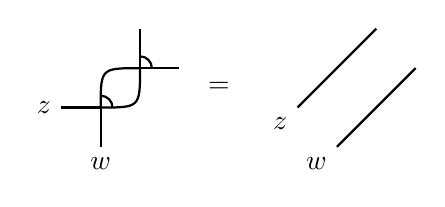
\begin{tikzpicture}
\draw (-0.5,0) -- (0,0);
\draw (0,-0.5) -- (0,0);
\draw (0.15,0) arc (0:90:0.15);
\draw (0.5,0.5) -- (1,0.5);
\draw (0.5,0.5) -- (0.5,1);
\draw (0.65,0.5) arc (0:90:0.15);
\draw (0,0) .. controls (0,0.5) .. (0.5,0.5);
\draw (0,0) .. controls (0.5,0) .. (0.5,0.5);
\node[left] at (-0.5,0) {$z$};
\node[below] at (0,-0.5) {$w$};

\node at (1.5,0.25) {$=$};

\draw (2.5,0) -- (3.5,1);
\draw (3,-0.5) -- (4,0.5);
\node[below left] at (2.5,0) {$z$};
\node[below left] at (3,-0.5) {$w$};
\end{tikzpicture}
\end{center}
which is essentially the second Reidemeister move. We can always switch from one convention to the other at the cost of normalization factors. The crucial difference between conventions lies in their analytic structure, which we will make use of extensively. More specifically:
\begin{align*}
1 &= R(\infty) = \lim_{z \to \infty} \mathcal{R}(z)/z = \check R(\infty), \\
P &= -\operatorname{Res}_{z=0} R(z)/\eta = -\mathcal{R}(0)/\eta = \check R(0), \\
\Pi^+ &= R(-\eta)/2 = -\mathcal{R}(-\eta)/2\eta = \check R(-\eta), \\
\Pi^- &= R(\eta)/2 = \mathcal{R}(\eta)/2\eta = \operatorname{Res}_{z=\eta} \check R(z)/2\eta,
\end{align*}
where $\Pi^\pm = (1 \pm P)/2$ are the symmetrizer and antisymmetrizer respectively. This is where the $R$-matrix becomes singular.
\end{remark}

\begin{definition}
\begin{enumerate}[label=(\roman*)]
\item For $y \in \C[\eta]$, the Yangian has the \emph{shift automorphism}
\begin{equation*}
\exp(-y\partial): Y(\mathfrak{gl}_\ell)[[z^{-1}]] \to Y(\mathfrak{gl}_\ell)[[z^{-1}]], \quad t_{ij}(z) \mapsto t_{ij}(z-y).
\end{equation*}
This is possible because we can expand $(z-y)^{-r}$ as a power series in $z^{-1}$:
\begin{equation*}
(z-y)^{-r} = \sum_{s=r}^\infty {s-1 \choose r-1} y^{s-r} z^{-s}.
\end{equation*}
\item There is the \emph{transposition automorphism} $T(z) \mapsto T^t(-z)$, or $t_{ij}(z) \mapsto t_{ji}(-z)$.
\item Given any $f(z) \in \C[\eta][[z^{-1}]]$ with leading term one, there is an automorphism $T(z) \mapsto f(z) T(z)$.
\item Given any $g \in \operatorname{GL}_\ell$, there is an automorphism $T(z) \mapsto g T(z) g^{-1}$.
\end{enumerate}
\end{definition}
 
\subsection{Representations of the Yangian}

We briefly recall the representation theory of $\mathfrak{gl}_\ell$ before moving on to the Yangian. Consider a representation $V$ of $U(\mathfrak{gl}_\ell)$. A non-zero element $\omega \in V$ is a highest weight vector with highest weight $\lambda = (\lambda_1,...,\lambda_\ell)$ for $\lambda_i \in \C$ if the following relations hold:
\begin{align*}
e_{ij} \omega &= 0, \quad 1 \leq i < j \leq \ell \\
e_{ii} \omega &= \lambda_i \omega, \quad 1 \leq i \leq \ell.
\end{align*}
If $V$ is generated by $\omega$, $V$ is a highest weight representation with highest weight $\lambda$. Clearly, any highest weight representation is a quotient of the Verma module $M(\lambda)$, which is defined as $U(\mathfrak{gl}_\ell)$ quotiented by the left ideal generated by the coefficients of $e_{ij}$ for $i<j$ as well as $e_{ii} - \lambda_i$. The Verma module has a unique maximal submodule, so that it has a unique simple quotient, which is denoted $L(\lambda)$. These are finite-dimensional if and only if $\lambda_i - \lambda_{i+1} \in \Z_+$ for $i=1,...,\ell-1$, which means that $\lambda$ can be thought of as a complex number $\lambda_1$ together with a Young diagram with at most $\ell$ rows, see appendix \ref{appendix:youngdiagrams} for more on Young diagrams. They exhaust all finite-dimensional irreducible polynomial representations of $U(\mathfrak{gl}_\ell)$.

We now proceed similarly with the Yangian:

\begin{definition}
Let $V$ be a representation of $Y(\mathfrak{gl}_\ell)$. A non-zero element $\omega \in V$ is of \emph{highest weight} $\lambda(z) = (\lambda_1(z),...,\lambda_\ell(z))$ for $\lambda_i(z) \in \C[\eta][[z^{-1}]]$ if the following relations hold:
\begin{align*}
t_{ij}(z) \omega &= 0, \quad 1 \leq i < j \leq \ell \\
t_{ii}(z) \omega &= \lambda_i(z) \omega, \quad 1 \leq i \leq \ell.
\end{align*}
If $V$ is generated by $\omega$, we call $V$ a \emph{highest weight representation} with highest weight $\lambda(z)$. Again, any highest weight representation is a quotient of the \emph{Verma module} $M(\lambda(z))$, which is just $Y(\mathfrak{gl}_\ell)$ quotiented by the left ideal generated by the coefficients of $t_{ij}(z)$ for $i<j$ as well as $t_{ii}(z) - \lambda_i(z)$. The Verma module has a unique maximal submodule, so that it has a unique simple quotient, which we denote by $L(\lambda(z))$.
\end{definition}

\begin{theorem}
Every finite-dimensional irreducible representation of $Y(\mathfrak{gl}_\ell)$ is a highest weight representation of the form $L(\lambda(z))$ for some highest weight $\lambda(z)$ and has a unique highest weight vector $\omega$ up to rescaling.
\end{theorem}

\begin{proof}
This is theorem 3.2.7 of \cite{book:molev}.
\end{proof}

\begin{theorem}
The irreducible highest weight representation $L(\lambda(z))$ of $Y(\mathfrak{gl}_\ell)$ is finite-dimensional if and only if
\begin{equation*}
\frac{\lambda_i(z)}{\lambda_{i+1}(z)} = \frac{p_i(z+\eta)}{p_i(z)}
\end{equation*}
for $i=1,...,\ell-1$ and unique monic polynomials $p_i(z) \in \C[\eta][z]$ called \emph{Drinfeld polynomials}.
\end{theorem}

\begin{proof}
This is theorem 3.4.1 of \cite{book:molev}. We consider the case $\ell = 2$. Essentially, one first finds a power series $f(z) \in \C[[z^{-1}]]$ such that $f(z) \lambda_1(z)$ and $f(z) \lambda_2(z)$ are polynomials, so that we can say without loss of generality that
\begin{equation*}
\lambda_1(z) = (1+\alpha_1 z^{-1}) \cdots (1+\alpha_k z^{-1}), \quad \lambda_2(z) = (1+\beta_1 z^{-1}) \cdots (1+\beta_k z^{-1}).
\end{equation*}
for certain complex numbers $\alpha_1,...,\alpha_k,\beta_1,...,\beta_k$. One shows that finite-dimensionality implies $(\alpha_i - \beta_i)/\eta \in \Z_+$ for all $i=1,...,k$ after some renumbering. Define the \emph{string}
\begin{equation*}
S(\alpha_i,\beta_i) := \{ \beta_i, \beta_i+\eta, ..., \alpha_i-2\eta, \alpha_i-\eta \}.
\end{equation*}
We now set
\begin{equation*}
p(z) := \prod_{i=1}^k \prod_{\gamma \in S(\alpha_i,\beta_i)} (z + \gamma),
\end{equation*}
which fulfills $\lambda_1(z) / \lambda_2(z) = p(z+\eta) / p(z)$ as can be seen by their poles and zeros.
\end{proof}

\begin{corollary}
Finite-dimensional irreducible representations of $Y(\mathfrak{gl}_\ell)$ are parametrized by tuples $(f(z),p_1(z),...,p_{\ell-1}(z))$ for $f(z)$ a power series in $z^{-1}$ with constant term one and $p_1(z),...,p_{\ell-1}(z)$ monic polynomials.
\end{corollary}

\begin{proof}
The $p_i(z)$ correspond to the Drinfeld polynomials and $f(z)$ to $\lambda_\ell(z)$.
\end{proof}

\begin{definition}
Given a weight $\lambda = (\lambda_1,...,\lambda_\ell) \in \C^\ell$ for $\mathfrak{gl}_\ell$, we can pull the irreducible representation $L(\lambda)$ of $\mathfrak{gl}_\ell$ back along the evaluation homomorphism. Due to surjectivity of the evaluation homomorphism, the resulting representation of $Y(\mathfrak{gl}_\ell)$ will still be irreducible and it will be a highest weight representation with highest weight components $\lambda_i(z) = 1 + \eta \lambda_i z^{-1}$. For simplicity, we also write $L(\lambda)$ for this $Y(\mathfrak{gl}_\ell)$-module. Such modules are called \emph{evaluation modules}\index{Evaluation module}. When they are finite-dimensional, they have Drinfeld polynomials
\begin{equation*}
p_i(z) = (z+\eta \lambda_{i+1})(z+\eta \lambda_{i+1}+\eta) \cdots (z+\eta \lambda_i-2\eta)(z+\eta \lambda_i-\eta),
\end{equation*}
which is makes sense due to $(\lambda_i - \lambda_{i+1})/\eta \in \Z_+$. We may twist evaluation modules by the shift automorphism for $y \in \C$ or the transposition and respectively obtain modules we denote by $L(\lambda)_y$ and $L(\lambda)^t$ as well as $L(\lambda)_y^t$.
\end{definition}

\begin{remark}
Let $y_1,...,y_N \in \C$ and consider a tensor product
\begin{equation*}
L(\lambda^{(1)})_{y_1}^t \otimes \cdots \otimes L(\lambda^{(N)})_{y_N}^t,
\end{equation*}
which inherits the structure of a $Y(\mathfrak{gl}_\ell)$-module via the coproduct. Let $\omega_j$ denote the highest weight vector of $L(\lambda^{(j)})_{y_j}^t$, respectively, and define $\omega := \omega_1 \otimes \cdots \otimes \omega_N$, which is a highest weight vector with highest weight components
\begin{equation*}
\lambda_i(z) := \left( 1 - \frac{\eta \lambda_i^{(1)}}{z-y_1} \right) \cdots \left( 1 - \frac{\eta \lambda_i^{(N)}}{z-y_N} \right).
\end{equation*}
Note that these weight components are not linear polynomials anymore. This is because such representations are genuine representations of $Y(\mathfrak{gl}_\ell)$, not of $\mathfrak{gl}_\ell$. Physically, this reflects the fact that local sites usually transform in representations of $\mathfrak{gl}_\ell$ while the extended Yangian symmetry acts non-locally, \emph{i.e.} on multiple tensorands. Hence, a large class of physically relevant representations of the Yangian are given by representations of this form:
\end{remark}

\begin{definition}
Representations of the form
\begin{equation*}
L(\lambda^{(1)})_{y_1}^t \otimes \cdots \otimes L(\lambda^{(N)})_{y_N}^t,
\end{equation*}
as above are called \emph{monodromy representations}\index{Monodromy representation} with \emph{inhomogeneities} $y_1,...,y_N$ and the highest weight vector $\omega$ is called the \emph{pseudovacuum}. 
\end{definition}

We now take a closer look at how transfer matrices act on monodromy representations. Our starting observation is the following:

\begin{lemma}
The generator matrix $T(z)$ acts on the evaluation module $L(\ydiagram{1})_y^t$ corresponding to the fundamental $\mathfrak{gl}_\ell$-representation $\C^\ell$ via the $R$-matrix:
\begin{equation*}
R(z-y) = 1 - \frac{\eta P}{z-y}.
\end{equation*}
\end{lemma}

\begin{proof}
Inserting the definition of evaluation modules, we see that $T(z)$ acts as
\begin{equation*}
\sum_{ij} e_{ij} \otimes \bigg( \delta_{ij} - \frac{\eta e_{ji}}{z-y} \bigg)
= \sum_{i} e_{ii} \otimes e_{ii} - \frac{\eta}{z-y} \sum_{ij} e_{ij} \otimes e_{ji} = 1 - \frac{\eta P}{z-y}.
\end{equation*}
\end{proof}

\begin{remark}
This shows that the RTT relation (\ref{equation:RTTRelation}) in the fundamental representation becomes the \emph{quantum Yang-Baxter equation}
\begin{equation*}
R_{12}(z-w) R_{13}(z) R_{23}(w) = R_{23}(w) R_{13}(z) R_{12}(z-w) \in \End (\C^\ell)^{\otimes 3},
\end{equation*}
where the subscript again denotes which spaces the $R$-matrix acts on. Diagrammatically, this reads
\begin{center}
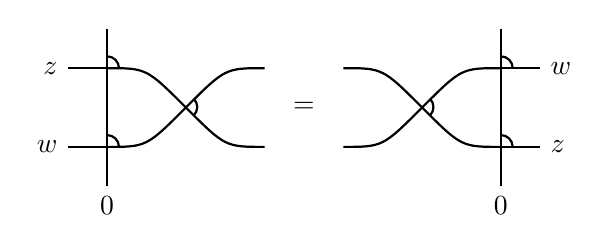
\begin{tikzpicture}
\draw (0,-0.5) -- (0,1.5);
\draw (-0.5,0) -- (0,0);
\draw (0.15,0) arc (0:90:0.15);
\draw (-0.5,1) -- (0,1);
\draw (0.15,1) arc (0:90:0.15);
\draw (0,0) .. controls (0.5,0) .. (1,0.5);
\draw (0,1) .. controls (0.5,1) .. (1,0.5);
\draw (1,0.5) .. controls (1.5,1) .. (2,1);
\draw (1,0.5) .. controls (1.5,0) .. (2,0);
\draw (1+.1,0.5-.1) arc (-45:45:0.15);
\node[left] at (-0.5,0) {$w$};
\node[left] at (-0.5,1) {$z$};
\node[below] at (0,-0.5) {$0$};

\node at (2.5,0.5) {$=$};

\draw (5,-0.5) -- (5,1.5);
\draw (5.5,0) -- (5,0);
\draw (5.15,0) arc (0:90:0.15);
\draw (5.5,1) -- (5,1);
\draw (5.15,1) arc (0:90:0.15);
\draw (5,0) .. controls (4.5,0) .. (4,0.5);
\draw (5,1) .. controls (4.5,1) .. (4,0.5);
\draw (4,0.5) .. controls (3.5,1) .. (3,1);
\draw (4,0.5) .. controls (3.5,0) .. (3,0);
\draw (4+.1,0.5-.1) arc (-45:45:0.15);
\node[right] at (5.5,0) {$z$};
\node[right] at (5.5,1) {$w$};
\node[below] at (5,-0.5) {$0$};
\end{tikzpicture}
\end{center}
which is the third Reidemeister move.
\end{remark}

Having $L(\ydiagram{1})_y^t$ under our belt, let us look at monodromy representations of the type
\begin{equation*}
L(\ydiagram{1})_{y_1}^t \otimes \cdots \otimes L(\ydiagram{1})_{y_N}^t,
\end{equation*}
which we call \emph{fundamental}.

\begin{prop}
The generator matrix $T(z)$ acts on fundamental monodromy representations via the \emph{monodromy matrix}
\begin{equation*}
M(z) := R_{0N}(z-y_N) \cdots R_{01}(z-y_1),
\end{equation*}
where $0$ is the auxiliary space index and $1,...,N$ are quantum space indices. In terms of diagrams, this reads
\begin{center}
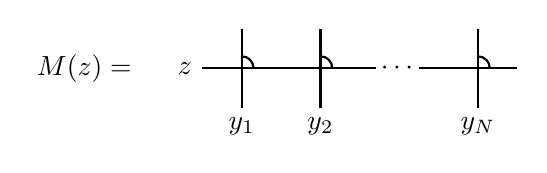
\begin{tikzpicture}
\node at (-2,0) {$M(z) =$};
\draw (-0.5,0) -- (0.5,0);
\draw (0,-0.5) -- (0,0.5);
\draw (0.15,0) arc (0:90:0.15);
\node[left] at (-0.5,0) {$z$};
\node[below] at (0,-0.5) {$y_1$};
\draw (0.5,0) -- (1.7,0);
\draw (1,-0.5) -- (1,0.5);
\draw (1.15,0) arc (0:90:0.15);
\node[below] at (1,-0.5) {$y_2$};
\node at (2,0) {$\cdots$};
\draw (2.25,0) -- (3.5,0);
\draw (3,-0.5) -- (3,0.5);
\draw (3.15,0) arc (0:90:0.15);
\node[below] at (3,-0.5) {$y_N$};
\end{tikzpicture}
\end{center}
\end{prop}

\begin{proof}
This follows from the previous lemma and the formula for the coproduct (\ref{equation:coproduct}), except the order is reversed since we used the transposition automorphism.
\end{proof}

\subsection{The Heisenberg model}

\begin{definition}
The \emph{twisted inhomogeneous Heisenberg $\mathfrak{gl}_\ell$-spin chain} of \emph{length} $N$ with invertible \emph{twist matrix} $g = \operatorname{diag}(\gamma_1,...,\gamma_\ell)$ and \emph{inhomogeneities $y_1,...,y_N$}, or \emph{Heisenberg model}\index{Heisenberg model} for short, has as Hilbert space the fundamental monodromy representations of the Yangian with inhomogeneities $y_1,...,y_N$. Here $\eta$ plays the role of Planck's constant. The generating function for the Hamiltonians is the \emph{$g$-twisted transfer matrix}\index{Transfer matrix}
\begin{equation*}
\tau^g(z) := \operatorname{tr}_0 g_0 T(z),
\end{equation*}
where $0$ denotes the auxiliary space index. In the fundamental monodromy representation, this takes the form
\begin{equation*}
\tau^g(z) = \operatorname{tr}_0 g_0 R_{0N}(z-y_N) \cdots R_{01}(z-y_1),
\end{equation*}
or, using the the unitary convention,
\begin{equation*}
\check \tau^g(z) = \operatorname{tr}_0 g_0 \check R_{0N}(z-y_N) \cdots \check R_{01}(z-y_1).
\end{equation*}
The corresponding diagram reads
~\\
\begin{center}
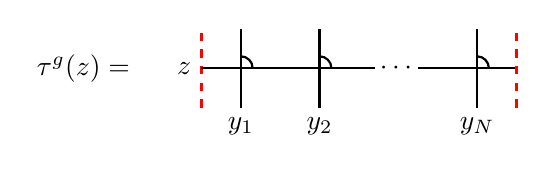
\begin{tikzpicture}
\draw[red,dashed] (-0.5,-0.5) -- (-0.5,0.5);
\node at (-2,0) {$\tau^g(z) =$};
\draw (-0.5,0) -- (0.5,0);
\draw (0,-0.5) -- (0,0.5);
\draw (0.15,0) arc (0:90:0.15);
\node[left] at (-0.5,0) {$z$};
\node[below] at (0,-0.5) {$y_1$};
\draw (0.5,0) -- (1.7,0);
\draw (1,-0.5) -- (1,0.5);
\draw (1.15,0) arc (0:90:0.15);
\node[below] at (1,-0.5) {$y_2$};
\node at (2,0) {$\cdots$};
\draw (2.25,0) -- (3.5,0);
\draw (3,-0.5) -- (3,0.5);
\draw (3.15,0) arc (0:90:0.15);
\node[below] at (3,-0.5) {$y_N$};
\draw[red,dashed] (3.5,-0.5) -- (3.5,0.5);
\end{tikzpicture}
\end{center}
where the dashed red lines indicate the twist matrix and are identified so that the whole diagram wraps around a cylinder, yielding the trace over the auxiliary space. One now defines commuting \emph{non-local Hamiltonians}\index{Non-local Hamiltonians} by
\begin{align*}
H_i 
&:= -\operatorname{Res}_{z=y_i} \tau^g(z)/\eta \\
&= \operatorname{tr}_0 g_0 R_{0N}(y_i-y_N) \cdots R_{0,i+1}(y_i-y_{i+1}) P_{0i} R_{0,i-1}(y_i-y_{i-1}) \cdots R_{01}(y_i-y_1) \\
&= \operatorname{tr}_0 R_{0,i-1}(y_i-y_{i-1}) \cdots R_{01}(y_i-y_1) g_0 R_{0N}(y_i-y_N) \cdots R_{0,i+1}(y_i-y_{i+1}) P_{0i} \\
&= \operatorname{tr}_0 P_{0i} R_{i,i-1}(y_i-y_{i-1}) \cdots R_{i1}(y_i-y_1) g_i R_{iN}(y_i-y_N) \cdots R_{i,i+1}(y_i-y_{i+1}) \\
&= R_{i,i-1}(y_i-y_{i-1}) \cdots R_{i1}(y_i-y_1) g_i R_{iN}(y_i-y_N) \cdots R_{i,i+1}(y_i-y_{i+1}),
\end{align*}
similarly
\begin{align*}
\check H_i
&:= \check \tau^g(y_i) = \bigg( \prod_{i \neq j} \frac{y_i-y_j}{y_i-y_j-\eta} \bigg) H_i \\
&= \check R_{i,i-1}(y_i-y_{i-1}) \cdots \check R_{i1}(y_i-y_1) g_i \check R_{iN}(y_i-y_N) \cdots \check R_{i,i+1}(y_i-y_{i+1}).
\end{align*}
As an example, for $i=2$, this yields the diagram
~\\
\begin{center}
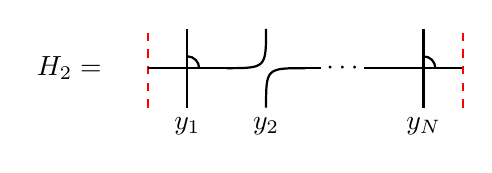
\begin{tikzpicture}
\draw[red,dashed] (-0.5,-0.5) -- (-0.5,0.5);
\node at (-1.5,0) {$H_2 =$};
\draw (-0.5,0) -- (0.5,0);
\draw (0,-0.5) -- (0,0.5);
\draw (0.15,0) arc (0:90:0.15);
\node[below] at (0,-0.5) {$y_1$};
\draw (0.5,0) .. controls (1,0) .. (1,0.5);
\draw (1,-0.5) .. controls (1,0) .. (1.5,0);
\draw (1.5,0) -- (1.7,0);
\node[below] at (1,-0.5) {$y_2$};
\node at (2,0) {$\cdots$};
\draw (2.25,0) -- (3.5,0);
\draw (3,-0.5) -- (3,0.5);
\draw (3.15,0) arc (0:90:0.15);
\node[below] at (3,-0.5) {$y_N$};
\draw[red,dashed] (3.5,-0.5) -- (3.5,0.5);
\end{tikzpicture}
\end{center}
To get a Hamiltonian describing local interactions, we have to restrict to $y_1,...,y_N = 0$. Define the operators
\begin{align*}
\mathcal{P} &:= g_1 P_{12} \cdots P_{N-1,N} \text{ and} \\
\mathcal{H} &:= -\sum_{i=1}^{N-1} P_{i,i+1} - g_1 P_{1N}.
\end{align*}
We call $\mathcal{P}$ the \emph{total momentum} and $\mathcal{H}$ the \emph{local Hamiltonian}\index{Local Hamiltonian}.
\end{definition}

\begin{prop}
Let $y_1,...,y_N = 0$. Then $\tau^g(z)$ has the following expansion around $z=0$:
\begin{equation*}
\tau^g(z) = \frac{\eta^N}{z^N} \mathcal{P} - \frac{\eta^{N-1}}{z^{N-1}} \mathcal{H} \mathcal{P} + \mathcal{O}(z^{-N+2})
\end{equation*}
\end{prop}

\begin{proof}
Let us expand $z^N \tau^g(z)$ around $z = 0$. To zeroth order, we have
\begin{align*}
z^N \tau^g(z)|_{z=0}
&= \eta^N \operatorname{tr}_0 g_0 P_{0N} \cdots P_{01} \\
&= \eta^N \operatorname{tr}_0 P_{0N} \cdots P_{01} g_0 \\
&= \eta^N \operatorname{tr}_0 P_{12} \cdots P_{N-1,N} g_N P_{0N} \\
&= \eta^N \operatorname{tr}_0 g_1 P_{12} \cdots P_{N-1,N} P_{0N} \\
&= \eta^N g_1 P_{12} \cdots P_{N-1,N} = \eta^N \mathcal{P}.
\end{align*}
To first order, we have
\begin{align*}
\frac{\partial}{\partial z} z^N \tau^g(z)|_{z=0}
&= \eta^{N-1} \sum_i \operatorname{tr}_0 g_0 P_{0N} \cdots P_{0,i+1} P_{0,i-1} \cdots P_{01} \\
&= \eta^{N-1} \sum_i \operatorname{tr}_0 P_{0N} \cdots P_{0,i+1} P_{0,i-1} \cdots P_{01} g_0 \\
&= \eta^{N-1} \sum_i \operatorname{tr}_0 P_{12} \cdots P_{i-1,i-2} P_{i-1,i+1} P_{i+1,i+2} \cdots P_{N-1,N} g_N P_{0N} \\
&= \eta^{N-1} \sum_i g_1 P_{12} \cdots P_{i-1,i-2} P_{i-1,i+1} P_{i+1,i+2} \cdots P_{N-1,N}.
\end{align*}
Now observe for $1 \leq i < N$:
\begin{align*}
& g_1 P_{12} \cdots P_{i-1,i-2} P_{i-1,i+1} P_{i+1,i+2} \cdots P_{N-1,N} \mathcal{P}^{-1} \\
&= g_1 P_{12} \cdots P_{i-2,i-1} P_{i-1,i+1} P_{i+1,i} P_{i,i-1} P_{i-1,i-2} \cdots P_{21} g_1^{-1} \\
&= P_{12} \cdots P_{i-2,i-1} P_{i-1,i+1} P_{i+1,i} P_{i,i-1} P_{i-1,i-2} \cdots P_{21} g_1 g_1^{-1} \\
&= P_{12} \cdots P_{i-2,i-1} P_{i-1,i+1} P_{i+1,i-1} P_{i+1,i} P_{i-1,i-2} \cdots P_{21} \\
&= P_{12} \cdots P_{i-2,i-1} P_{i+1,i} P_{i-1,i-2} \cdots P_{21} = P_{i,i+1},
\end{align*}
while $i=N$ gives $g_1 P_{1N}$ (tba). Hence $z^N \tau(z) = \eta^N \mathcal{P} - z \eta^{N-1} \mathcal{H} \mathcal{P} + \mathcal{O}(z^2)$.
\end{proof}

In the case $\ell=2$, we can further rewrite this in a way that makes apparent how the Hamiltonian of the Heisenberg model describes twisted-periodic alignment of nearest neighbor spins, \emph{i.e.} ferromagnetic materials:

\begin{corollary}
Let $\ell = 2$ and $\sigma^x,\sigma^y,\sigma^z$ be the Pauli matrices. Then
\begin{align*}
\mathcal{H} = &- \frac{N-1}{2} - \frac{1}{2} \sum_{i=1}^{N-1} \left( \sigma_i^x \sigma_{i+1}^x + \sigma_i^y \sigma_{i+1}^y + \sigma_i^z \sigma_{i+1}^z \right) \\
&- \frac{1}{2} g_1 - \frac{1}{2} \left( g_1\sigma_1^x \sigma_N^x + g_1 \sigma_1^y \sigma_N^y + g_1 \sigma_1^z \sigma_N^z \right).
\end{align*}
\end{corollary}

\begin{proof}
This follows from the identity $1 + \sigma^x \otimes \sigma^x + \sigma^y \otimes \sigma^y + \sigma^z \otimes \sigma^z = 2P$.
\end{proof}

%%%%%%%%%%%%%%%%%%%%%%%%%%%%%%%%%%%%%%%%%

\chapter{Duality} \label{chapter:duality}

\section{Quantum-classical duality from functional relations}

There is an enormous body of work on solving the Heisenberg model, \emph{i.e.} diagonalizing its Hamiltonians, by various loosely related methods. Prime focus is given to a variety of approaches called \emph{Bethe ansätze}, particularly the algebraic Bethe ansatz, see \cite{book:arutyunov:betheAnsatz}, which produces eigenvectors from the pseudovacuum using ladder operators supplemented by auxiliary equations called \emph{Bethe equations}. In the coming sections, we will focus on an orthogonal approach employing functional relations between transfer matrices. This approach is originally due to \cite{article:kuniba:1994} and has been further developed in \cite{book:arutyunov:betheAnsatz}, where it is shown how the Lax matrix of the classical rational Ruijsenaars-Schneider model secretly controls the fusion relations, giving a first hint of quantum-classical duality.

\subsection{Functional relations}

Our key to solving the Heisenberg model is to enlargen our consideration of the $g$-twisted transfer matrix $\tau^g(z)$ to a big commutative subalgebra that contains it and make use of functional relations inside this subalgebra to arrive at a set of polynomial equations, the \emph{spectral equation}, that the eigenvalues of the non-local Hamiltonians $H_1,...,H_N$, \emph{i.e.} the residues of $\tau^g(z)$, must satisfy. To this end, we consider the \emph{Bethe subalgebra}:

\begin{definition}
The \emph{$g$-twisted Bethe subalgebra}\index{Bethe subalgebra} is the subalgebra $B^g(\mathfrak{gl}_\ell)$ of $Y(\mathfrak{gl}_\ell)$ generated by the coefficients of the higher $g$-twisted transfer matrices $\tau_\lambda^g(z)$, where $\lambda$ ranges over Young diagrams.
\end{definition}

\begin{theorem}
The Bethe subalgebra $B^g(\mathfrak{gl}_\ell)$ is a maximal commutative subalgebra of $Y(\mathfrak{gl}_\ell)$ whenever $g$ has simple spectrum.
\end{theorem}

\begin{proof}
This appears in \cite{article:nazarov:1996}.
\end{proof}

Now, we have left out what we mean by the higher $g$-twisted transfer matrices $\tau_\lambda^g(z)$. The basic idea is to take the definition of the usual transfer matrix and switch the auxiliary space from the fundamental representation to a higher representation labeled by a Young diagram $\lambda$. This gives rise to the higher transfer matrices $\tau_\lambda^g(z)$. In particular of course, $\tau_{\ydiagram{1}}^g(z)$ will coincide with the usual transfer matrix.

\begin{definition}
Let $\lambda$ be a Young diagram. Let $g_\lambda,(e_{ij})_\lambda \in \operatorname{End} L(\lambda)$ denote the action of the twist matrix and the matrix units on the highest weight representation $L(\lambda)$. Define the \emph{higher $g$-twisted transfer matrix of shape $\lambda$}\index{Higher transfer matrix}
\begin{equation*}
\tau_\lambda^g(z) := \operatorname{tr}_\lambda g_\lambda T_\lambda(z), \quad T_\lambda(z) = \sum_{ij} (e_{ij})_\lambda \otimes t_{ij}(z).
\end{equation*}
\end{definition}

The functional relations between higher transfer matrices come from the so called \emph{fusion relations}\index{Fusion procedure}, which categorify into short exact sequences of representations of the Yangian. Of particular importance will be the following short exact sequence:
\begin{equation*}
0 \to L([2,1^{k-1}])_0^t \to L([1^k])_0^t \otimes L(\ydiagram{1})_\eta^t \to L([1^{k+1}])_\eta^t \to 0.
\end{equation*}
The analogous sequence for $\mathfrak{sl}_2$ was originally established in \cite{article:chari:1990}. In terms of Young diagrams, the case $k=3$ simply reads
\begin{equation*}
\ydiagram{1,1,1} \otimes \ydiagram{1} = \ydiagram{2,1,1} \oplus \ydiagram{1,1,1,1},
\end{equation*}
which is the usual Littlewood-Richardson rule, except crucially we have an added dependence on the parameter $z$, which makes this short exact sequence non-split in general. Finally, the rule for traces over short exact sequences will give the functional relation
\begin{equation*}
\tau_{[1^k]}^g(z) \tau_{\ydiagram{1}}^g(z+\eta) = \tau_{[2,1^{k-1}]}^g(z) + \tau_{[1^{k+1}]}^g(z+\eta),
\end{equation*}
which will be our basis for deriving the spectral equation.

Let us now set out to show this, starting with a discussion of the \emph{fusion procedure} \cite{article:molev:2008}, originating in works such as \cite{article:kulish:1981}. To this end, fix a standard Young tableau $t_\lambda$ of shape $\lambda$ with content vector $(c_1,...,c_k)$ and let
\begin{equation*}
R(z_1,...,z_k) := \overset{\longrightarrow}{\prod_{i<j}} R_{ij}(z_i-z_j),
\end{equation*}
where the arrow over the product indicates multiplication in lexicographical order. We note that successive application of the RTT relation (\ref{equation:RTTRelation}) yields
\begin{equation}\label{equation:higherRTT}
R(z_1,...,z_k) T_1(z_1) \cdots T_k(z_k) = T_k(z_k) \cdots T_1(z_1) R(z_1,...,z_k).
\end{equation}

\begin{prop}\label{prop:fusionDecomposition}
Taking the following consecutive limits of $R(z_1,...,z_k)$ yields a well-defined \emph{fusion projector}
\begin{equation*}
\Pi_{t_\lambda} = \frac{d_\lambda}{k!} \lim_{z_k \to \eta c_k} \cdots \lim_{z_1 \to \eta c_1} R(z_1,...,z_k),
\end{equation*}
with $d_\lambda$ the dimension of the Specht module $S(\lambda)$ given by the hook formula. The fusion projectors form a complete set of primitive orthogonal idempotents decomposing the $\mathfrak{gl}_\ell$-module $(\C^\ell)^{\otimes k}$ into irreducible parts
\begin{equation*}
L_{t_\lambda} := \Pi_{t_\lambda} (\C^\ell)^{\otimes k}
\end{equation*}
with $L_{t_\lambda} \cong L(\lambda)$ as $\mathfrak{gl}_\ell$-modules.
\end{prop}

\begin{proof}
See \cite{article:molev:2008} or section 6.4 in \cite{book:molev}.
\end{proof}

\begin{prop}
Let $t_\lambda$ be a standard Young tableau of shape $\lambda$ with content vector $(c_1,...,c_k)$ and consider $(\C^\ell)^{\otimes k}$ as the monodromy representation
\begin{equation*}
L(\ydiagram{1})_{\eta c_1}^t \otimes \cdots \otimes L(\ydiagram{1})_{\eta c_k}^t.
\end{equation*}
Then $L_{t_\lambda} \cong L(\lambda)_0^t$ as $Y(\mathfrak{gl}_\ell)$-modules.
\end{prop}

\begin{proof}
This is proposition 6.5.1 in \cite{book:molev}.
\end{proof}

This procedure makes it possible to reduce calculations in higher representations to tensor products of the fundamental representation. It is called the \emph{fusion procedure}. In particular, we can express higher transfer matrices in a very concrete way using $(\C^\ell)^{\otimes k}$ as the auxiliary space. To see this, define
\begin{equation*}
T_{t_\lambda}(z) := T_k(z+\eta c_k) \cdots T_1(z+\eta c_1), \quad g_{t_\lambda} := g_k \cdots g_1.
\end{equation*}
Then $L_{t_\lambda} \otimes Y(\mathfrak{gl}_\ell)[[z^{-1}]]$ is invariant under $g_{t_\lambda} T_{t_\lambda}(z)$ due to
\begin{equation*}
\Pi_{t_\lambda} T_1(z+\eta c_1) \cdots T_k(z+\eta c_k) = T_k(z+\eta c_k) \cdots T_1(z+\eta c_1) \Pi_{t_\lambda},
\end{equation*}
which is derived from the higher RTT relation (\ref{equation:higherRTT}) by taking consecutive limits. It follows that

\begin{prop}
We have the identity
\begin{equation*}
\tau_\lambda^g(z) = \operatorname{tr}_{t_\lambda} g_{t_\lambda} T_{t_\lambda}(z)
\end{equation*}
where $\operatorname{tr}_{t_\lambda}$ denotes the partial trace over $L_{t_\lambda}$.
\end{prop}

\begin{example}
Consider $\tau_{[1^2]}^g(z)$. With the previous proposition, we can write this as
\begin{equation*}
\tau_{[1^2]}^g(z) = \operatorname{tr}_{t_{[1^2]}} g_{t_{[1^2]}} T_{t_{[1^2]}}(z) = \operatorname{tr}_{12} \Pi_{t_{[1^2]}} g_2 g_1 T_2(z) T_1(z-\eta).
\end{equation*}
In particular, in the fundamental monodromy representation $L(\ydiagram{1})_{y_1}^t \otimes L(\ydiagram{1})_{y_2}^t$, this becomes
\begin{equation*}
\tau_{[1^2]}^g(z) = \operatorname{tr}_{12} \Pi_{12}^- g_2 g_1 R_{23}(z-y_1) R_{24}(z-y_2) R_{13}(z-\eta-y_1) R_{14}(z-\eta-y_2).
\end{equation*}
In terms of diagrams, this reads
~\\
\begin{center}
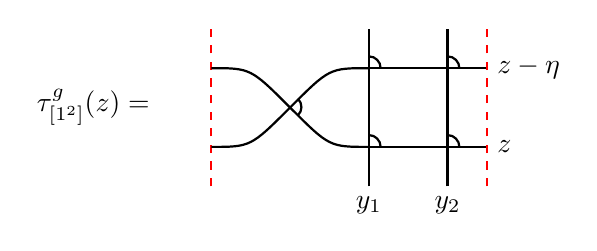
\begin{tikzpicture}
\node at (1.5,0.5) {$\tau_{[1^2]}^g(z) =$};
\draw[red,dashed] (3,-0.5) -- (3,1.5);
\draw (5,-0.5) -- (5,1.5);
\draw (6,-0.5) -- (6,1.5);
\draw (6.5,0) -- (5,0);
\draw (5.15,0) arc (0:90:0.15);
\draw (6.15,0) arc (0:90:0.15);
\draw (6.5,1) -- (5,1);
\draw (5.15,1) arc (0:90:0.15);
\draw (6.15,1) arc (0:90:0.15);
\draw (5,0) .. controls (4.5,0) .. (4,0.5);
\draw (5,1) .. controls (4.5,1) .. (4,0.5);
\draw (4,0.5) .. controls (3.5,1) .. (3,1);
\draw (4,0.5) .. controls (3.5,0) .. (3,0);
\draw (4+.1,0.5-.1) arc (-45:45:0.15);
\node[right] at (6.5,0) {$z$};
\node[right] at (6.5,1) {$z-\eta$};
\node[below] at (5,-0.5) {$y_1$};
\node[below] at (6,-0.5) {$y_2$};
\draw[red,dashed] (6.5,-0.5) -- (6.5,1.5);
\end{tikzpicture}
\end{center}
Note that the auxiliary space loops twice around the cylinder, exactly shifting by $\pm \eta$ when crossing the seam.
\end{example}

We can now also see that the highest transfer matrix $\tau_{[1^\ell]}^g(z)$ has a particularly nice description in terms of a Leibniz-type formula:

\begin{corollary}
\begin{equation*}
\tau_{[1^\ell]}^g(z) = \sum_\sigma \operatorname{sgn} \sigma \cdot \gamma_1 \gamma_2 \cdots \gamma_\ell \cdot t_{\sigma(1) 1}(z) t_{\sigma(2) 2}(z-\eta) \cdots t_{\sigma(\ell) \ell}(z-\eta (\ell-1)).
\end{equation*}
\end{corollary}

\begin{proof}
From the previous proposition, we have
\begin{equation*}
\tau_{[1^\ell]}^g(z) = \operatorname{tr}_{t_{[1^\ell]}} g_{t_{[1^\ell]}} T_{t_{[1^\ell]}}(z) = \operatorname{tr}_{1,...,\ell} \Pi_{t_{[1^\ell]}} g_k \cdots g_1 T_\ell(z-\eta(\ell-1)) \cdots T_1(z).
\end{equation*}
Noting that $\Pi_{t_{[1^\ell]}} = \sum_\sigma \operatorname{sgn} \sigma \cdot \sigma$, we apply the right hand side to $e_1 \otimes \cdots \otimes e_\ell$ and obtain
\begin{equation*}
\sum_{i_1,...,i_\ell} \Pi_{t_{[1^\ell]}} (e_{i_1} \otimes \cdots \otimes e_{i_\ell}) \otimes t_{i_1,1}(z) t_{i_2,2}(z-\eta) \cdots t_{i_\ell,\ell}(z-\eta(\ell-1)).
\end{equation*}
But $\Pi_{t_{[1^\ell]}} (\gamma_{i_1} e_{i_1} \otimes \cdots \otimes \gamma_{i_\ell} e_{i_\ell})$ is only non-zero when the $i_1,...,i_\ell$ define a permutation $\sigma$, in which case it reduces to $\operatorname{sgn} \sigma \cdot \gamma_1 \cdots \gamma_\ell (e_1 \otimes \cdots \otimes e_\ell)$.
\end{proof}

\begin{definition}
Due to this fact, $\tau_{[1^\ell]}^g(z)$ deserves the name \emph{$g$-twisted quantum determinant}\index{Quantum determinant}. We hence also write 
\begin{equation*}
\operatorname{qdet}^g T(z) := \tau_{[1^\ell]}^g(z).
\end{equation*}
\end{definition}

\begin{prop}
The center of $Y(\mathfrak{gl}_\ell)$ is freely generated by the coefficients of $\operatorname{qdet}^g T(z)$.
\end{prop}

\begin{proof}
This is theorem 1.7.5 in \cite{book:molev}.
\end{proof}

\begin{corollary}\label{corollary:quantumDet}
Let $V$ be a highest weight representation of $Y(\mathfrak{gl}_\ell)$ with highest weight $\lambda(z) = (\lambda_1(z),...,\lambda_\ell(z))$. Then $\operatorname{qdet}^g T(z)$ acts as a scalar of the form
\begin{equation*}
\gamma_1 \gamma_2 \cdots \gamma_\ell \lambda_1(z) \lambda_2(z-\eta) \cdots \lambda_\ell(z-\eta(\ell-1)).
\end{equation*}
\end{corollary}

\begin{proof}
This is proposition 3.2.5 of \cite{book:molev}. Since $T(z)$ acts as a lower-triangular matrix on the highest weight vector, the only non-zero term in the Leibniz formula above is the term for $\sigma = \id$, which acts exactly as described. Since $\operatorname{qdet}^g T(z)$ lies in the center of $Y(\mathfrak{gl}_\ell)$, it will act on all vectors of $V$ via this scalar.
\end{proof}

\begin{prop}
The transfer matrices $\tau_\lambda^g(z)$ commute among each other, making $B^g(\mathfrak{gl}_\ell)$ into a commutative algebra.
\end{prop}

\begin{proof}
tba
\end{proof}

To finish off this section, let us finally prove the exactness of our sequence:

\begin{prop}
There is an exact sequence
\begin{equation*}
0 \to L([2,1^{k-1}])_0^t \to L([1^k])_0^t \otimes L(\ydiagram{1})_\eta^t \to L([1^{k+1}])_\eta^t \to 0.
\end{equation*}
\end{prop}

\begin{proof}
Consider the fundamental monodromy representation
\begin{equation*}
L(\ydiagram{1})_0^t \otimes L(\ydiagram{1})_{-\eta}^t \otimes \cdots \otimes L(\ydiagram{1})_{-\eta(k-1)}^t \otimes L(\ydiagram{1})_1^t.
\end{equation*}
By the previous proposition, the fusion projectors $\Pi_{t_{[2,1^{k-1}]}}$ and $\Pi_{t_{[1^k]}} \otimes 1$ project onto the left and middle pieces $L([2,1^{k-1}])_0^t$ and $L([1^k])_0^t \otimes L(\ydiagram{1})_1^t$. The Littlewood-Richardson rule gives
\begin{equation*}
\Pi_{t_{[1^k]}} \otimes 1 = \Pi_{t_{[2,1^{k-1}]}} + \Pi_{t_{[1^{k+1}]}},
\end{equation*}
so that $\Pi_{t_{[2,1^{k-1}]}}$ actually factors through $\Pi_{t_{[1^k]}} \otimes 1$, which yields the inclusion from the left to the middle piece. Then $\Pi_{t_{[1^{k+1}]}}$ will be the projection onto the cokernel of this inclusion. The RTT relation supplemented by $\Pi_{t_{[1^{k+1}]}} \Pi_{t_{[1^k]}} = \Pi_{t_{[1^{k+1}]}}$ gives
\begin{align*}
&\Pi_{t_{[1^{k+1}]}} R_{01}(z) R_{02}(z-\eta) \cdots R_{0k}(z-\eta(k-1)) R_{0,k+1}(z+\eta) \\
&= \Pi_{t_{[1^{k+1}]}} \Pi_{t_{[1^k]}} R_{01}(z) R_{02}(z-\eta) \cdots R_{0k}(z-\eta(k-1)) R_{0,k+1}(z+\eta) \\
&= \Pi_{t_{[1^{k+1}]}} R_{0k}(z-\eta(k-1)) \cdots R_{02}(z-\eta) R_{01}(z) R_{0,k+1}(z+\eta) \Pi_{t_{[1^k]}} \\
&= R_{0,k+1}(z+\eta) R_{01}(z) R_{02}(z-\eta) \cdots R_{0k}(z-\eta(k-1)) \Pi_{t_{[1^{k+1}]}} \Pi_{t_{[1^k]}} \\
&= R_{0,k+1}(z+\eta) R_{01}(z) R_{02}(z-\eta) \cdots R_{0k}(z-\eta(k-1)) \Pi_{t_{[1^{k+1}]}},
\end{align*}
so $\Pi_{t_{[1^{k+1}]}}$ is in fact $Y(\mathfrak{gl}_\ell)$-linear, as required.
\end{proof}

\begin{corollary}
We obtain the functional relation
\begin{equation}\label{equation:functionalRelation}
\tau_{[1^k]}^g(z) \tau_{\ydiagram{1}}^g(z+\eta) = \tau_{[2,1^{k-1}]}^g(z) + \tau_{[1^{k+1}]}^g(z+\eta).
\end{equation}
\end{corollary}

\begin{proof}
By the previous proposition, we have a morphism of short exact sequences: \\
{\small
\begin{tikzcd}[column sep=0.3cm]
\\
0 \arrow{r}
& L([2,1^{k-1}])_0 \otimes Y(\mathfrak{gl}_\ell)[[z^{-1}]] \arrow{r} \arrow{d}{g_{[2,1^{k-1}]} T_{[2,1^{k-1}]}(z)}
& L([1^k])_0 \otimes L(\ydiagram{1})_\eta \otimes Y(\mathfrak{gl}_\ell)[[z^{-1}]] \arrow{r} \arrow{d}{g_{[1^k]} T_{[1^k]}(z) g_{\ydiagram{1}} T_{\ydiagram{1}}(z+\eta)}
& L([1^{k+1}])_\eta \otimes Y(\mathfrak{gl}_\ell)[[z^{-1}]] \arrow{r} \arrow{d}{g_{[1^{k+1}]} T_{[1^{k+1}]}(z+\eta)}
& 0 \\
0 \arrow{r}
& L([2,1^{k-1}])_0 \otimes Y(\mathfrak{gl}_\ell)[[z^{-1}]] \arrow{r}
& L([1^k])_0 \otimes L(\ydiagram{1})_\eta \otimes Y(\mathfrak{gl}_\ell)[[z^{-1}]] \arrow{r}
& L([1^{k+1}])_\eta \otimes Y(\mathfrak{gl}_\ell)[[z^{-1}]] \arrow{r}
& 0 \\
\end{tikzcd}
}
Taking the trace over everything except $Y(\mathfrak{gl}_\ell)[[z^{-1}]]$ yields
\begin{equation*}
0 = \tau_{[2,1^{k-1}]}^g(z) - \tau_{[1^k]}^g(z) \tau_{\ydiagram{1}}^g(z+\eta) + \tau_{[1^{k+1}]}^g(z+\eta)
\end{equation*}
as elements of $Y(\mathfrak{gl}_\ell)[[z^{-1}]]$.
\end{proof}

\subsection{Spectral equation}

In this section, we will derive the \emph{spectral equation} for the non-local Hamiltonians of the Heisenberg model from the functional relation established earlier. This is where we will see the Lax matrix of the rational Ruijsenaars-Schneider model appear seemingly out of nowhere. The rest of this thesis is dedicated to explaining this occurrence. We will work along the lines of \cite{book:arutyunov:betheAnsatz}, but our approach is slightly different since we use Yang's convention for $R$-matrices.

\begin{lemma}
We have
\begin{equation*}
\operatorname{Res}_{z=y_i} \tau_{[1^{k+1}]}^g(z)
= \chi_{[1^k]}(g) H_i + \sum_j \frac{\eta H_i}{y_i-y_j-\eta} \operatorname{Res}_{z=y_j} \tau_{[1^k]}^g(z).
\end{equation*}
\end{lemma}

\begin{proof}
We take the residue of the functional relation (\ref{equation:functionalRelation}) and arrive at
\begin{equation*}
\operatorname{Res}_{z=y_i} \tau_{[1^{k+1}]}^g(z)
= \tau_{[1^k]}^g(y_i-\eta) \operatorname{Res}_{z=y_i} \tau_{\ydiagram{1}}^g(z),
\end{equation*}
where we have used
\begin{equation*}
\operatorname{Res}_{z=y_i} \tau_{[2,1^{k-1}]}^g(z-\eta) = 0.
\end{equation*}
tba
\end{proof}

In matrix notation, this reads
\begin{equation*}
\begin{pmatrix}
\operatorname{Res}_{z=y_1} \tau_{[1^{k+1}]}^g(z) \\
\vdots \\
\operatorname{Res}_{z=y_N} \tau_{[1^{k+1}]}^g(z)
\end{pmatrix}
=
\chi_{[1^k]}(g)
\begin{pmatrix}
H_1 \\
\vdots \\
H_N
\end{pmatrix}
-L^t
\begin{pmatrix}
\operatorname{Res}_{z=y_1} \tau_{[1^k]}^g(z) \\
\vdots \\
\operatorname{Res}_{z=y_N} \tau_{[1^k]}^g(z)
\end{pmatrix}
\end{equation*}
with
\begin{equation*}
L_{ij} := \frac{\eta H_j}{y_i-y_j+\eta} = \frac{\eta}{y_i-y_j+\eta} \bigg( \prod_{j \neq k} \frac{y_j-y_k-\eta}{y_j-y_k} \bigg) \check H_j.
\end{equation*}
This looks awfully close to the Lax matrix (\ref{equation:RSLaxMatrix}) of the rational Ruijsenaars-Schneider model! Iterating and combining with corollary \ref{corollary:quantumDet} finally gives the spectral equation, resembling a Cayley-Hamilton-type identity:

\begin{theorem}[Spectral equation]\label{theorem:spectralEq}
The non-local Hamiltonians $H_1,...,H_N$ of the spin chain fulfill the \emph{spectral equation}
\begin{equation*}
\chi_{[1^\ell]}(g)
\begin{pmatrix}
\operatorname{Res}_{z=y_1} \operatorname{qdet}^1 T(z) \\ \vdots \\ \operatorname{Res}_{z=y_N} \operatorname{qdet}^1 T(z)
\end{pmatrix}
= \sum_{k=1}^\ell \chi_{[1^{\ell-k}]}(g) (-L^t)^{k-1}
\begin{pmatrix}
H_1 \\ \vdots \\ H_N
\end{pmatrix}
\end{equation*}
\end{theorem}

\begin{proof}
tba
\end{proof}

\begin{corollary}
The eigenvalues of $H_1,...,H_N$ are exactly the complex roots of the spectral equation.
\end{corollary}

\begin{proof}
?? tba
\end{proof}

\section{Generalized Schur-Weyl duality}

Why should the Lax matrix of the rational Ruijsenaars-Schneider model appear in the spectral equation? A first clue is given by the fact that the Yangian allows for residual symmetries through its various automorphisms, the most peculiar of which is the shift automorphism. It has no analogue for $\mathfrak{gl}_\ell$ and is thus special to the Yangian. This non-rigidity gives additional degrees of freedom for monodromy representations: the inhomogeneities. These seem to play the role of the position variables of the rational Ruijsenaars-Schneider model. What is the mathematical reason for their appearance? Most simply, it is because the Schur-Weyl dual of the Yangian is the degenerate affine Hecke algebra, whose generators include polynomial generators that act as inhomogeneities. To introduce this, we will start with a discussion of classical Schur-Weyl duality between the symmetric groups $S_N$ and the Lie algebras $\mathfrak{gl}_\ell$. A detailed account of various generalized Schur-Weyl dualities can be found in \cite{thesis:antor:2020}.

\subsection{Classical Schur-Weyl duality}

Classical Schur-Weyl duality establishes a link between the representation theory of the symmetric group $S_N$ and the representation theory of the Lie algebra $\mathfrak{gl}_\ell$. Let $\C^\ell$ be the fundamental representation of $\mathfrak{gl}_\ell$ and consider the $N$-fold tensor product representation $(\C^\ell)^{\otimes N}$. Clearly, $\mathfrak{gl}_\ell$ acts from the left via the coproduct of $U(\mathfrak{gl}_\ell)$. However, there is also a right action of $S_N$ by permuting tensorands. Schur-Weyl duality now states the following:

\begin{theorem}
The actions of $U(\mathfrak{gl}_\ell)$ and $\C[S_N]$ on $(\C^\ell)^{\otimes N}$ are each others centralizer.\index{Schur-Weyl duality}
\end{theorem}

\begin{corollary}
We have the decomposition
\begin{equation*}
(\C^\ell)^{\otimes N} = \bigoplus_{\lambda} L(\lambda) \otimes S(\lambda),
\end{equation*}
where $\lambda$ ranges over all Young diagrams with $N$ boxes and at most $\ell$ rows, $L(\lambda)$ is the corresponding irreducible highest weight representation of $\mathfrak{gl}_\ell$ and $S(\lambda)$ is the corresponding Specht module of $S_N$, compare proposition \ref{prop:fusionDecomposition}.
\end{corollary}

\begin{corollary}
We have $L(\lambda) = (\C^\ell)^{\otimes N} \otimes_{S_N} S(\lambda)$.
\end{corollary}

The last part can be nicely organized in categorical language, following \cite{article:davydov:2010}. Define a monoidal category $S_*$ with objects $[N]$ for $N \in \N$ and monoidal product $[N] \otimes [M] := [N+M]$ as well as morphisms
\begin{equation*}
\Hom_{S_*}([N],[M]) :=
\begin{cases}
\C[S_N], & N = M \\
\varnothing, & N \neq M
\end{cases}
\end{equation*}
with the monoidal product of morphisms given by the natural map $\C[S_N] \otimes \C[S_M] \to \C[S_{N+M}]$. We now take the following $\C$-linear closure
\begin{equation*}
\mathsf{C}(S_*) := [S_*,\mathsf{Vect}] \simeq \bigoplus_N \C[S_N]\mathsf{Mod},
\end{equation*}
where we have a tensor product given by Day convolution:
\begin{equation*}
V \otimes_{S_*} W := \C[S_{N+M}] \otimes_{\C[S_N] \otimes \C[S_M]} (V \otimes W).
\end{equation*}
which gives a monoidal fiber functor
\begin{equation*}
F_\ell: \mathsf{C}(S_*) \to \mathsf{Vect}, \quad V \in \C[S_N]\mathsf{Mod} \mapsto (\C^\ell)^{\otimes N} \otimes_{S_N} V.
\end{equation*}
The fact that $U(\mathfrak{gl}_\ell)$ centralizes the action of the symmetric groups gives a homomorphism $U(\mathfrak{gl}_\ell) \to \End(F_\ell)$ and we obtain a commutative diagram
\begin{center}
\begin{tikzcd}
\mathsf{C}(S_*) \arrow[swap]{dr}{SW_\ell} \arrow{rr}{F_\ell} & & \mathsf{Vect} \\
& U(\mathfrak{gl}_\ell)\mathsf{Mod} \arrow{ur}
\end{tikzcd}
\end{center}
Hence we may say that the algebras $U(\mathfrak{gl}_\ell)$ are Tannaka dual to the algebras $\C[S_N]$.

\begin{theorem}[Classical Schur-Weyl duality]
The functor
\begin{equation*}
SW_{\ell,N}: \C[S_N]\mathsf{Mod} \to U(\mathfrak{gl}_\ell)\mathsf{Mod}, \quad V \mapsto (\C^\ell)^{\otimes N} \otimes_{S_N} V
\end{equation*}
is full and faithful when $\ell \geq N$. Its essential image are $U(\mathfrak{gl}_\ell)$-modules of weight $N$.
\end{theorem}

\subsection{Schur-Weyl duality for the Yangian}

The important observation now is that classical Schur-Weyl duality may be generalized from the Lie algebra $\mathfrak{gl}_\ell$ to the Yangian $Y(\mathfrak{gl}_\ell)$ by replacing the symmetric group with the degenerate affine Hecke algebra. The additional action by shifts of the spectral parameter $z$ of the Yangian is defined using the action of the polynomial generators $y_i$ of the degenerate affine Hecke algebra.

Proceeding as above, following the language of \cite{article:davydov:2010}, we define a monoidal category $\dot H_*$ with objects $[N]$ for $N \in \N$, monoidal product $[N] \otimes [M] := [N+M]$ as well as morphisms
\begin{equation*}
\Hom_{\dot H_*}([N],[M]) :=
\begin{cases}
\dot H_N, & N = M \\
\varnothing, & N \neq M
\end{cases}
\end{equation*}
with the monoidal product of morphisms given by the natural map $\dot H_N \otimes \dot H_M \to \dot H_{N+M}$. We again take the $\C$-linear closure
\begin{equation*}
\mathsf{C}(\dot H_*) := [\dot H_*,\mathsf{Vect}] \simeq \bigoplus_N \dot H_N\mathsf{Mod},
\end{equation*}
equipped with the tensor product
\begin{equation*}
V \otimes_{\dot H_*} W := \dot H_{N+M} \otimes_{\dot H_N \otimes \dot H_M} (V \otimes W).
\end{equation*}
We may define a fiber functor $\mathsf{C}(\dot H_*) \to \mathsf{Vect}$ that factors through a functor $D_\ell: \mathsf{C}(\dot H_*) \to Y(\mathfrak{gl}_\ell)\mathsf{Mod}$. Its components are called \emph{Drinfeld functors}.

\begin{definition}
We define the \emph{Drinfeld functor}
\begin{equation*}
D_{\ell,N}: \dot H_N\mathsf{Mod} \to Y(\mathfrak{gl}_\ell)\mathsf{Mod}, \quad V \mapsto (\C^\ell)^{\otimes N} \otimes_{S_N} V
\end{equation*}
by first considering the case $N=1$ and introducing a $Y(\mathfrak{gl}_\ell)$-module structure on the tensor product $\C^\ell \otimes V$ via
\begin{equation*}
t_{ij}^{(r)}(u \otimes v) := -\eta e_{ji} u \otimes y_1^{r-1} v,
\end{equation*}
which becomes
\begin{equation*}
t_{ij}(z) \mapsto \delta_{ij} - \frac{\eta e_{ji}}{z-y_1} \quad \text{or} \quad T(z) \mapsto R(z-y_1)
\end{equation*}
in power series and matrix notation, respectively. The coproduct of the Yangian extends the definition to the remaining cases $N > 1$:
\begin{equation*}
T(z) \mapsto R_{0N}(z-y_N) \cdots R_{01}(z-y_1).
\end{equation*}
\end{definition}

\begin{theorem}[Schur-Weyl duality for the Yangian]
The Drinfeld functor is full and faithful when $\ell > N$. Its essential image are $Y(\mathfrak{gl}_\ell)$-modules of weight $N$.
\end{theorem}

\begin{proof}
This is the main theorem of \cite{article:drinfeld:1986}. Drinfeld's original proof has never been published, but \cite{article:chari:1995} contains a detailed and long-winded proof for the analogous case of affine quantum groups.
\end{proof}

\begin{prop}
The Drinfeld functor is a monoidal functor in the following sense:
\begin{equation*}
D_{\ell,N+M}(V \otimes_{\dot H_*} W) = D_{\ell,N}(V) \otimes D_{\ell,M}(W).
\end{equation*}
\end{prop}

We can already see how this is beginning to resemble the structure we are looking for: The Drinfeld functor takes representations of the degenerate affine Hecke algebra $\dot H_N$, such as the wave function representation of the quantum rational Ruijsenaars-Schneider model, and produces a representation of the Yangian clearly resembling fundamental monodromy representations with inhomogeneities given by the polynomial generators $y_i$ of the degenerate affine Hecke algebra. More precisely, when $\mathfrak{m} = (y_1-\bar y_1,...,y_N-\bar y_N)$ for complex numbers $\bar y_i$, we have an isomorphism
\begin{equation*}
D_{\ell,N}(\C[y_1,...,y_N]) \otimes_{\C[y_1,...,y_N]} \C[y_1,...,y_N]/\mathfrak{m} \cong L(\ydiagram{1})_{\bar y_1}^t \otimes \cdots \otimes L(\ydiagram{1})_{\bar y_N}^t
\end{equation*}
of $Y(\mathfrak{gl}_\ell)$-modules. However, we are still missing two important ingredients: Firstly, the twist matrix does not enter into the structure at any point, and secondly, we are disregarding the Laurent generators $X_i$ of the degenerate double affine Hecke algebra $\ddot H_N$, which play an important role in defining the Hamiltonians of the quantum rational Ruijsenaars-Schneider model. These shortcomings will be remedied in the next section.

\subsection{Twisted Schur-Weyl duality for the Yangian}

It is clear that any $\ddot H_N$-module restricts to an $\dot H_N$-module to which we can apply the Drinfeld functor, giving a new functor
\begin{equation*}
\ddot H_N\mathsf{Mod} \to Y(\mathfrak{gl}_\ell)\mathsf{Mod}, \quad V \mapsto (\C^\ell)^{\otimes N} \otimes_{S_N} V.
\end{equation*}
Crucially however, we still have the action of the Laurent generators $X_i$ on $(\C^\ell)^{\otimes N} \otimes_{S_N} V$ left over. Since we tensor over the symmetric group, we are required to restrict to operators that are symmetric in the $X_i$. Such operators are provided by the spherical degenerate double affine Hecke algebra $S\ddot H_N$. Naively incorporating this action yields a functor
\begin{equation*}
\ddot H_N\mathsf{Mod} \to S\ddot H_N \# Y(\mathfrak{gl}_\ell)\mathsf{Mod}.
\end{equation*}
Let us now twist this using the twist matrix $g$:

\begin{definition}
Define the \emph{preaffine Drinfeld functor}
\begin{equation*}
D_{\ell,N}^g: \ddot H_N\mathsf{Mod} \to S\ddot H_N \# Y(\mathfrak{gl}_\ell)\mathsf{Mod}, \quad V \mapsto (\C^\ell)^{\otimes N} \otimes_{S_N} V,
\end{equation*}
by letting $X_i$ act on $(\C^\ell)^{\otimes N} \otimes_{S_N} V$ via
\begin{equation*}
X_i(u \otimes v) := g_i u \otimes X_i v.
\end{equation*}
The $y_i$ act untwisted.
\end{definition}

With this definition, we are finally ready to show explicitly how the preaffine Drinfeld functor maps the quantum rational Ruijsenaars-Schneider model to the twisted inhomogeneous Heisenberg model in the limit $\hbar \to 0$. This is the aim of the next section.

\section{Quantum-classical duality as Schur-Weyl duality}

\subsection{Fundamental spin chain}

In this section, we will show how the wave function representation $\C[y_1,...,y_N]$ of the quantum rational Ruijsenaars-Schneider model produces the the fundamental spin chain, \emph{i.e.}
\begin{equation*}
L(\ydiagram{1})_{y_1}^t \otimes \cdots \otimes L(\ydiagram{1})_{y_N}^t
\end{equation*}
via the preaffine Drinfeld functor. Our first step is a simple but powerful observation:

\begin{lemma}
On $(\C^\ell)^{\otimes N} \otimes_{S_N} \C[y_1,...,y_N]$, we have
\begin{equation*}
g_i u \otimes X_i f = \check R_{i,i-1}(y_i-y_{i-1}) \cdots \check R_{i1}(y_i-y_1) (g_i \otimes e^{\I \hbar \partial_i}) \check R_{iN}(y_i-y_N) \cdots \check R_{i,i+1}(y_i-y_{i+1}) (u \otimes f).
\end{equation*}
where
\begin{equation*}
\check R_{ij}(y_i-y_j) (u \otimes f) := u \otimes \frac{y_i-y_j}{y_i-y_j-\eta} f - u s_i \otimes \frac{\eta}{y_i-y_j-\eta} f.
\end{equation*}
\end{lemma}

\begin{proof}
Since we are tensoring over $S_N$, we know that $u s_i \otimes f = u \otimes T_i f$, \emph{i.e.}
\begin{align*}
us_i  \otimes f &= u \otimes \bigg( \frac{y_i-y_{i+1}-\eta}{y_i-y_{i+1}} s_i + \frac{\eta}{y_i-y_{i+1}} \bigg) f \\
\Leftrightarrow u s_i \otimes f - u \otimes \frac{\eta}{y_i-y_{i+1}} f &= u \otimes \frac{y_i-y_{i+1}-\eta}{y_i-y_{i+1}} s_i f \\
\Leftrightarrow u s_i \otimes \frac{y_i-y_j}{y_i-y_j-\eta} f - u \otimes \frac{\eta}{y_i-y_j-\eta} f &= u \otimes s_i f,
\end{align*}
or in short:
\begin{equation*}
\check R_{i,i+1}(y_i-y_{i+1}) (u s_i \otimes f) = u \otimes s_i f.
\end{equation*}
In combination, we obtain
\begin{equation*}
u \otimes x_{i,i+1} f = u \otimes s_i T_i f = \check R_{i,i+1}(y_i-y_{i+1}) (u s_i \otimes T_i f) = \check R_{i,i+1}(y_i-y_{i+1})(u \otimes f).
\end{equation*}
It follows that
\begin{align*}
g_i u \otimes X_i f
&= g_i u \otimes x_{i,i-1} \cdots x_{i1} e^{\I \hbar \partial_i} x_{iN} \cdots x_{i,i+1} f \\
&= \check R_{i,i-1}(y_i-y_{i-1}) \cdots \check R_{i1}(y_i-y_1) (g_i u \otimes e^{\I \hbar \partial_i} x_{iN} \cdots x_{i,i+1} f) \\
&= \check R_{i,i-1}(y_i-y_{i-1}) \cdots \check R_{i1}(y_i-y_1) (g_i \otimes e^{\I \hbar \partial_i}) (u \otimes x_{iN} \cdots x_{i,i+1} f) \\
&= \check R_{i,i-1}(y_i-y_{i-1}) \cdots \check R_{i1}(y_i-y_1) (g_i \otimes e^{\I \hbar \partial_i}) \check R_{iN}(y_i-y_N) \cdots \check R_{i,i+1}(y_i-y_{i+1}) (u \otimes f).
\end{align*}
\end{proof}

\begin{corollary}
The operator
\begin{equation*}
\sum_j \frac{\eta}{z-y_j} \bigg( \prod_{k \neq j} \frac{y_j-y_k-\eta}{y_j-y_k} \bigg) X_j \in (S\ddot H_N)_{\delta(y)}[[z^{-1}]]
\end{equation*}
acts on $(\C^\ell)^{\otimes N} \otimes_{S_N} \C[y_1,...,y_N]$ as the transfer matrix $\tau^g(z)$ when $\hbar = 0$.
\end{corollary}

\begin{proof}
tba
\end{proof}

\begin{corollary}
In the classical limit, $\check H_i$ and $X_i$ act in the same way. It follows that
\begin{equation*}
L_{ij} = \frac{\eta H_i}{y_i-y_j+\eta} = \frac{\eta}{y_i-y_j+\eta} \bigg( \prod_{k \neq j} \frac{y_j-y_k-\eta}{y_j-y_k} \bigg) X_j = L_{ij}^\textnormal{RS}.
\end{equation*}
as well as
\begin{equation*}
\operatorname{tr} (L_{ij}^\textnormal{RS})^k = \sum_i M_i \gamma_i^k.
\end{equation*}
\end{corollary}

\begin{proof}
tba
\end{proof}

Let us finish by giving a Rosetta stone for quantum-classical duality:
\begin{center}
\begin{tabular}{|r||l|}
\hline
twisted inhomogeneous Heisenberg model & rational Ruijsenaars-Schneider model \\
\hline
Yangian $Y(\mathfrak{gl}_\ell)$ & degenerate affine Hecke algebra $\dot H_N$ \\
fundamental monodromy representation & wave function representation \\
$i$th atom & $i$th particle \\
inhomogeneities $y_i$ & positions $y_i$ \\
non-local Hamiltonians $\check H_i$ & Macdonald operators $X_i$ \\
twist parameters $\gamma_i$ & eigenvalues of the Lax matrix $L^\textnormal{RS}$ \\
residue at $\infty$ of transfer matrix $\tau^g(z)$ & Hamiltonian $\operatorname{tr} L^\textnormal{RS}$ \\
Planck constant $\eta$ & coupling constant $\eta$ \\
\hline
\end{tabular}
\end{center}

\subsection{Higher spin chain}

The way we have introduced the duality between the Heisenberg and Ruijsenaars-Schneider models easily lends itself to a generalization to spins in non-fundamental representations. Consider a Young diagram $\lambda$. We know that we can obtain the evaluation module $L(\lambda)_y^t$ as a submodule of the fundamental monodromy representation
\begin{equation*}
L(\ydiagram{1})_{y+\eta c_1}^t \otimes \cdots \otimes L(\ydiagram{1})_{y+\eta c_N}^t
\end{equation*}
by the fusion procedure with corresponding projector $\Pi_{t_\lambda}$, up to a choice of tableau $t_\lambda$ with content vector $(c_1,...,c_N)$. On the particle side, the projector $\Pi_{t_\lambda}$ similar corresponds to a projector and the positions of particles get restricted to $y_i = y + \eta c_i$. Physically, this means that spins in higher representations labeled by $\lambda$ do not correspond to single particles, but to a bound state of $N$ particles, where $N$ is the number of boxes of the Young diagram $\lambda$. The exact correspondence is found in \cite{article:arakawa:1999}.

\begin{example}
Let us look at the two site spin chain
\begin{equation*}
L(\ydiagram{2})_{y_1}^t \otimes L(\ydiagram{2})_{y_2}^t \subseteq L(\ydiagram{1})_{y_1}^t \otimes L(\ydiagram{1})_{y_1+\eta}^t \otimes L(\ydiagram{1})_{y_2}^t \otimes L(\ydiagram{1})_{y_2+\eta}^t.
\end{equation*}
with projector
\begin{equation*}
\Pi_{\ydiagram{2}} = (1 + (1 \ 2))/2.
\end{equation*}
Solving this with the spectral equation derived earlier proves difficult, since its coefficients become singular during fusion. However, solving the Wronskian equation \cite{book:arutyunov:betheAnsatz} for the $N=4$ $\mathfrak{gl}_2$ spin chain with generic inhomogeneities and performing the fusion procedure as well as going to the homogeneous limit yields the solution
\begin{equation*}
(z-\eta)^2 (2 z^2 + 4 \eta z + 4 \eta^2)
\end{equation*}
for the $\ydiagram{4}$-multiplet, which is exactly correct up to the factor $(z-\eta)^2$, which results from using the polynomial convention.
\end{example}

\begin{center}
\begin{tabular}{|r||l|}
\hline
twisted inhomogeneous Heisenberg model & rational Ruijsenaars-Schneider model \\
\hline
$i$th atom with spin in representation $\lambda^{(i)}$ & $i$th bound state of particles \\
\vdots & \vdots \\
\hline
\end{tabular}
\end{center}

\section{$S$-duality}

\subsection{Schur-Weyl duality for the loop Yangian}

Let us reexamine the preaffine Drinfeld functor
\begin{equation*}
D_{\ell,N}^g: \ddot H_N\mathsf{Mod} \to S\ddot H_N \# Y(\mathfrak{gl}_\ell) \mathsf{Mod}.
\end{equation*}
Note that there is an asymmetry in its definition: It prioritizes the polynomial generators $y_i$ by incorporating them in the action of the Yangian, while the $S$-dual Laurent generators $X_i$ are artificially added on. It is known that there is a generalized Schur-Weyl duality between the affine symmetric group, which is the source of the Laurent generators, and the loop algebra $L(\mathfrak{gl}_\ell) := U(\mathfrak{gl}_\ell[t^{\pm 1}])$\index{Loop algebra}. Thus, we might hope to put both sides on a more equal footing by incorporating an action of the loop algebra on $(\C^\ell)^{\otimes N} \otimes_{S_N} V$ in addition to the action of the Yangian, making use of the Laurent generators $X_i$:
\begin{equation*}
(x t^r)(u \otimes v) := \sum_i x_i u \otimes X_i^r v.
\end{equation*}
This yields an action of the $\C[\eta,\hbar]$-algebra $L(\mathfrak{gl}_\ell) \# Y(\mathfrak{gl}_\ell)$ on $(\C^\ell)^{\otimes N} \otimes_{S_N} V$. This action in fact descends to the \emph{loop Yangian $LY(\mathfrak{gl}_\ell)$}\index{Loop Yangian}, which is a quotient of $L(\mathfrak{gl}_\ell) \# Y(\mathfrak{gl}_\ell)$:

\begin{prop}
The action of the Yangian $Y(\mathfrak{gl}_\ell)$ and the loop algebra $L(\mathfrak{gl}_\ell)$ glue together to an action of the loop Yangian $LY(\mathfrak{gl}_\ell)$.
\end{prop}

\begin{proof}
This is proved in \cite{article:guay:2005}, also see \cite{article:kodera:2016}.
\end{proof}

\begin{definition}
This defines the \emph{affine Drinfeld functor}
\begin{equation*}
\dot D_{\ell,N}: \ddot H_N\mathsf{Mod} \to LY(\mathfrak{gl}_\ell) \mathsf{Mod}.
\end{equation*}
\end{definition}

We can now identify the Hamiltonians of the quantum rational Ruijsenaars-Schneider model and the quantum trigonometric Calogero-Moser model as elements of the loop Yangian:

\begin{prop}
On $(\C^\ell)^{\otimes N} \otimes_{S_N} \C[y_1,...,y_N]$, we have
\begin{equation*}
t(u \otimes f) = u \otimes D_1 f,
\end{equation*}
where $D_1$ is the Hamiltonian of the quantum rational Ruijsenaars-Schneider model.
\end{prop}

\begin{proof}
tba
\end{proof}

\begin{prop}
On $(\C^\ell)^{\otimes N} \otimes_{S_N} \C[X_1^{\pm 1},...,X_N^{\pm 1}]$, the quantum determinant has the following expansion:
\begin{align*}
\operatorname{qdet}^1 T(z)
= 1 &- \frac{\eta}{z} N - \frac{\eta}{z^2} \bigg( -\I \hbar \sum_i X_i \partial_i + \eta \frac{N(N-1)}{2} \bigg) \\
&- \frac{\eta}{z^3} \bigg( S_2 - \I \hbar \eta (N-1) \sum_i X_i \partial_i + \eta^2 \frac{N(N-1)(N-2)}{4} \bigg)
\end{align*}
\end{prop}

\begin{proof}
tba, see \cite{article:bernard:1993}.
\end{proof}

\subsection{The trigonometric Gaudin model}

The trigonometric Gaudin Hamiltonians should be represented by the Lax matrix
\begin{equation*}
G(t) = g_0 + \eta \sum_i \frac{tP_{0i}}{t-X_i},
\end{equation*}
for which the residues of $\frac{1}{2} \operatorname{tr} G(t)^2$ should give rise to Hamiltonians
\begin{equation*}
G_i := g_i + \eta \sum_{i \neq j} \frac{X_i P_{ij}}{X_i-X_j},
\end{equation*}
which is almost like a Dunkl operator:
\begin{equation*}
G_i - \eta \sum_{j < i} P_{ij} = g_i - \eta \sum_{j < i} \theta_{ji} P_{ij} + \eta \sum_{j > i} \theta_{ij} P_{ij}
\end{equation*}
\begin{equation*}
G_i - \eta \sum_{j < i} P_{ij} - \eta - \eta \sum_{i \neq j} \theta_{ij} =
g_i - i\eta + \eta \sum_{j < i} \theta_{ji} (1-P_{ij}) - \eta \sum_{j > i} \theta_{ij} (1-P_{ij})
\end{equation*}

The transfer matrix has the expansion
\begin{equation*}
\tau^1(z) = 1 - \frac{\eta}{z} N - \frac{\eta}{z^2} \bigg( \sum_i y_i - \eta \sum_{j<i} P_{ij} \bigg) + \mathcal{O}(z^{-3})
\end{equation*}

tba

\chapter{Geometry}\label{chapter:geometry}

\section{The geometry behind quantum-classical duality}

\subsection{In terms of functorial quantum field theory}

The aim of this section is to reformulate Schur-Weyl duality for the Yangian in terms of a 2-functorial quantum field theory that will turn out to represent four-dimensional Chern-Simons theory. The mathematical structures used so far have been heavily representation theoretical. Nonetheless, we have seen some hints that there is an underlying geometry at play: We have made use of braids on cylinders as well as complex coordinates that may be reinterpreted as $N$-pointed Riemann spheres. The foundation for our construction is a symmetric monoidal double category $2\mathsf{Cob}$ that unifies the data of Riemann spheres and braids on cylinders. Regarding symmetric monoidal double categories we follow the reference \cite{article:hansen:2019}, where they were originally defined as a tool for efficiently organizing the structure of symmetric monoidal bicategories.

\begin{definition}
\begin{enumerate}[label=(\roman*)]
\item A \emph{double category} $\mathsf{D}$ consists of a category of objects $\mathsf{D}^0$ and a category of morphisms $\mathsf{D}^1$ together with identity, source, target, and composition functors
\begin{equation*}
I: \mathsf{D}^0 \to \mathsf{D}^1, \quad S,T: \mathsf{D}^1 \to \mathsf{D}^0, \quad \bullet: \mathsf{D}^1 \times_{\mathsf{D}^0} \mathsf{D}^1 \to \mathsf{D}^1
\end{equation*}
as well as associator, left unitor, and right unitor isomorphisms
\begin{equation*}
\alpha: (C \bullet D) \bullet E \to C \bullet (D \bullet E), \quad \lambda: I \bullet C \to C, \quad \rho: C \bullet I \to C,
\end{equation*}
such that $SI = TI = \operatorname{Id}_{\mathsf{D}^0}$, $S(\alpha), T(\alpha), S(\lambda), T(\lambda), S(\rho), T(\rho)$ are all identities, $\alpha$ fulfills the pentagon axiom, and $\lambda, \rho$ fulfill the left and right unit axiom.
\item The morphisms of $\mathsf{D}^0$ are called \emph{tight morphisms}, written $f: M \to N$, while the objects of $\mathsf{D}^1$ are called \emph{loose morphisms}, written $C: S(C) \dashrightarrow T(C)$. A morphism $\beta: C \to D$ of $\mathsf{D}^1$ is called a \emph{square}, written
\begin{center}
\begin{tikzcd}[row sep=0.1cm,column sep=0.1cm]
S(C) \arrow[swap]{dd}{S(\beta)} \arrow[dashed]{rr}{C} & & T(C) \arrow{dd}{T(\beta)} \\
& \beta & \\
S(D) \arrow[dashed,swap]{rr}{D} & & T(D)
\end{tikzcd}
\end{center}
A square is \emph{globular} when both $S(\beta)$ and $T(\beta)$ are identities.
\item A \emph{double functor} $F: \mathsf{D} \to \mathsf{E}$ consists of two functors $F^0: \mathsf{D}^0 \to \mathsf{E}^0$ and $F^1: \mathsf{D}^1 \to \mathsf{E}^1$ such that $SF^1 = F^0S$, $TF^1 = F^0T$ and globular natural isomorphisms $F^\bullet: F^1 C \bullet F^1 D \to F^1(C \bullet D)$ subject to some coherence conditions.
\item A \emph{double natural transformation} $\nu: F \Rightarrow G: \mathsf{D} \to \mathsf{E}$ consists of two natural transformations $\nu^0: F^0 \Rightarrow G^0$ and $\nu^1: F^1 \Rightarrow G^1$ subject to some coherence conditions.
\item A \emph{symmetric monoidal double category} $\mathsf{D}$ is a double category such that $\mathsf{D}^0$ and $\mathsf{D}^1$ are both symmetric monoidal categories, $I$ maps the monoidal unit of $\mathsf{D}^0$ to the monoidal unit of $\mathsf{D}^1$, $S$ and $T$ are strict symmetric monoidal together with globular natural isomorphisms realizing the interchange law between $\bullet$ and $\otimes$ subject to some coherence conditions.
\item A \emph{strong symmetric monoidal double functor} $F: \mathsf{D} \to \mathsf{E}$ is a double functor such that $F^0$ and $F^1$ are strong symmetric monoidal functors together with double natural isomorphisms $\otimes \circ (F,F) \to F \circ \otimes$ and $I \to FI$ subject to some coherence conditions.
\end{enumerate}
\end{definition}

\begin{example}
Let $k$ be a commutative ring. There is the symmetric monoidal double category $k\mathsf{Alg}$ of $k$-algebras with
\begin{align*}
k\mathsf{Alg}^0 &:= \{ k\text{-algebras} \}, \\
k\mathsf{Alg}^1 &:= \{ (A,M,B) \mid A,B \text{ are } k\text{-algebras and } M \text{ is an } A\text{-}B\text{-bimodule} \}.
\end{align*}
Morphisms $f: A \to A'$ in $k\mathsf{Alg}^0$ are algebra homomorphisms and morphisms $\beta: (A,M,B) \to (A',M',B')$ in $k\mathsf{Alg}^1$ are triples $(f,\beta,g)$ with $f: A \to A', g: B \to B'$ algebra homomorphisms and $\beta: M \to M'$ a $k$-linear map with
\begin{equation*}
\beta(amb) = f(a) \beta(m) g(b).
\end{equation*}
Then $I$ sends a $k$-algebra $A$ to the regular $A$-$A$-bimodule and an algebra homomorphism $f: A \to A'$ to the triple $(f,f,f)$. On the other hand, $S$ and $T$ send $(A,M,B)$ to $A$ and $B$ and a morphism $(f,\beta,g): (A,M,B) \to (A',M',B')$ to $f$ and $g$, respectively. The $\bullet$-composition is defined as follows: Given
\begin{center}
\begin{tikzcd}[column sep=2cm]
A \arrow{r}{(A,M,B)} & B \arrow{r}{(B,N,C)} & C
\end{tikzcd}
\end{center}
we let $(B,N,C) \bullet (A,M,B)$ be the tensor product $(A,M \otimes_B N,C)$ over $B$ with the $A$-$C$-bimodule structure
\begin{equation*}
a(m \otimes n)c := am \otimes nc.
\end{equation*}
The symmetric monoidal structure on $k\mathsf{Alg}^0$ is given by the tensor product of algebras over $k$ and the symmetric monoidal structure on $k\mathsf{Alg}^1$ is given by the the following tensor product:
\begin{equation*}
(A,M,B) \otimes (A',M',B') := (A \otimes_k A',M \otimes_k M',B \otimes_k B'),
\end{equation*}
where $M \otimes_k M'$ has the $(A \otimes_k A')$-$(B \otimes_k B')$-bimodule structure
\begin{equation*}
(a \otimes a')(m \otimes m')(b \otimes b') := amb \otimes a'm'b'.
\end{equation*}
The standard braidings then make $k\mathsf{Alg}$ into a symmetric monoidal double category \cite{article:hansen:2019}.
\end{example}

\begin{definition}
\begin{enumerate}[label=(\roman*)]
\item The \emph{category of finite pointed sets} consists of finite sets with a distinguished element and maps that preserve distinguished elements. Canonical representatives of the isomorphism classes are given by $[N] := \{ \infty,1,...,N \}$ with $\infty$ distinguished.
\item Let $A$ be a pointed set. An \emph{$A$-pointed curve} $C$ is a complex projective curve together with pairwise distinct non-singular points $y_a \in C$ and non-zero tangent vectors $v_a \in T_{y_a} C$ indexed by $a \in A$. Let us write these data as $(C;(y_a)_{a \in A};(v_a)_{a \in A})$.
\item A \emph{morphism of $A$-pointed curves}
\begin{equation*}
f: (C;(y_a)_{a \in A};(v_a)_{a \in A}) \to (C';(y_{a})_{a \in A};(v_{a})_{a \in A})
\end{equation*}
is a morphism of complex projective curves $m: C \to C'$ such that $m(y_a) = y_{b(a)}'$ and $dm_{y_a}(v_a) = v_{b(a)}'$.
\item We let $M_{g,[N]}$ denote the set of isomorphism classes of $[N]$-pointed curves of genus $g$.
\item A \emph{smooth family $(C_t)_{0 \leq t \leq 1}$ of $[N]$-pointed curves} is a smooth path in $M_{*,[N]}$ fixing the first point. We remark that such a path can be visualized as a framed braid in the unpointed curve.
\item The \emph{complex Teichmüller groupoid $\mathcal{T}eich_{g,[N]}^\C$} has as objects $[N]$-pointed curves of genus $g$ and as morphisms $C \to C'$ smooth families $(C_t)_{0 \leq t \leq 1}$ of $[N]$-pointed curves together with isomorphisms $\varphi_0: C \to C_0$ and $\varphi_1: C' \to C_1$ modulo homotopy fixing the first point.
\end{enumerate}
\end{definition}

\begin{example}
Let $(C;y_\infty,...,y_N;v_\infty,...,v_N)$ be an $[N]$-pointed curve of genus zero. Then $C \cong \P^1$ and the automorphisms of $\P^1$ are known to be of the form
\begin{equation*}
\mu_A: \P^1 \to \P^1, \quad z \mapsto \frac{az+b}{cz+d}, \quad
A =
\begin{pmatrix}
a & b \\ c & d
\end{pmatrix}
\in \operatorname{SL}_2(\C).
\end{equation*}
This defines a 3-transitive action of $\operatorname{SL}_2(\C)$ on $\P^1$ and allows us to give a representative
\begin{equation*}
(C;y_\infty,y_1,...,y_N;v_\infty,v_1,...,v_N) \cong (\P^1;\infty,y_1,y_2,...,y_N;-\partial_{1/z},v_1,...,v_N)
\end{equation*}
of the isomorphism class, which still has one degree of freedom given by translation by $y \in \C$, represented via the matrix
\begin{equation*}
\begin{pmatrix}
1 & y \\ 0 & 1
\end{pmatrix}
\in \operatorname{SL}_2(\C).
\end{equation*}
Letting $\text{Conf}_N := \{ (y_1,...,y_N) \mid y_1,...,y_N \in \C, y_i \neq y_j \}$ be the configuration space of $N$ ordered points in the complex plane, we conclude that
\begin{equation*}
M_{0,[N]} \cong \C \backslash \text{Conf}_N \times (\C^\times)^N,
\end{equation*}
where we have quotiented by the action of $\C$ by translation.
\end{example}

\begin{definition}
The double category $2\mathsf{Cob}$ has as $2\mathsf{Cob}^0$ the core of the category of finite pointed sets and as $2\mathsf{Cob}^1$ the category whose objects are of the form $C: [N] \dashrightarrow [M]$ with $C$ an $[N] \sqcup [M]$-pointed curve and whose morphisms
\begin{center}
\begin{tikzcd}[column sep=3.5cm]
{[N]} \arrow{d}{\sigma} \arrow[dashed]{r}{(C;y_\infty,y_1,...,y_{N+M})} & {[M]} \arrow{d}{\tau} \\
{[N]} \arrow[dashed,swap]{r}{(C';y_\infty',y_1',...,y_{N+M}')} & {[M]}
\end{tikzcd}
\end{center}
are homotopy classes of smooth families $(C_t)_{0 \leq t \leq 1}$ of $[N] \sqcup [M]$-pointed curves with isomorphisms $C_0 \cong C$ and $C_1 \cong C'$ such that $y_i$ connects to $y_{(\sigma \sqcup \tau)(i)}'$.
\end{definition}

\begin{prop}
There is a double functor $2\mathsf{Cob} \to \C[\eta]\mathsf{Alg}$ mapping a pointed set $[N]$ to $Y(\mathfrak{gl}_\ell)^{\otimes N}$, a pointed permutation $\sigma: [N] \to [N]$ to the corresponding permutation on tensor factors, a genus zero curve $(\P^1;\infty,y_1,...,y_N;-\partial_{1/z},v_1,...,v_N)$ to the fundamental monodromy representation $L(\ydiagram{1})_{y_1}^t \otimes \cdots \otimes L(\ydiagram{1})_{y_N}^t$, shifts as
\begin{center}
\begin{tikzcd}[column sep=3.5cm]
{[N]} \arrow{d}{\id} \arrow[dashed]{r}{(\P^1;\infty,y_1,...,y_{N+M})} & {[M]} \arrow{d}{\id} \\
{[N]} \arrow[dashed,swap]{r}{(\P^1;\infty,y_1',...,y_{N+M}')} & {[M]}
\end{tikzcd}
$\quad \mapsto \quad$
\begin{tikzcd}[column sep=4cm]
Y(\mathfrak{gl}_\ell)^{\otimes N} \arrow{d}{\textnormal{shift}} \arrow[dashed]{r}{L(\ydiagram{1})_{y_1}^t \otimes \cdots \otimes L(\ydiagram{1})_{y_{N+M}}^t} & Y(\mathfrak{gl}_\ell)^{\otimes M} \arrow{d}{\textnormal{shift}} \\
Y(\mathfrak{gl}_\ell)^{\otimes N} \arrow[dashed,swap]{r}{L(\ydiagram{1})_{y_1'}^t \otimes \cdots \otimes L(\ydiagram{1})_{y_{N+M}'}^t} & Y(\mathfrak{gl}_\ell)^{\otimes M}
\end{tikzcd}
\end{center}
with the identity bimodule map, braids as
\begin{center}
\begin{tikzcd}[column sep=3.5cm]
{[N]} \arrow{d}{\sigma} \arrow[dashed]{r}{(\P^1;\infty,y_1,...,y_{N+M})} & {[M]} \arrow{d}{\tau} \\
{[N]} \arrow[dashed,swap]{r}{(\P^1;\infty,y_1,...,y_{N+M})} & {[M]}
\end{tikzcd}
$\quad \mapsto \quad$
\begin{tikzcd}[column sep=4cm]
Y(\mathfrak{gl}_\ell)^{\otimes N} \arrow{d}{\sigma} \arrow[dashed]{r}{L(\ydiagram{1})_{y_1}^t \otimes \cdots \otimes L(\ydiagram{1})_{y_{N+M}}^t} & Y(\mathfrak{gl}_\ell)^{\otimes M} \arrow{d}{\tau} \\
Y(\mathfrak{gl}_\ell)^{\otimes N} \arrow[dashed,swap]{r}{L(\ydiagram{1})_{y_1}^t \otimes \cdots \otimes L(\ydiagram{1})_{y_{N+M}}^t} & Y(\mathfrak{gl}_\ell)^{\otimes M}
\end{tikzcd}
\end{center}
with $b_i$ getting mapped to the $R$-matrix $\check R_{i,i+1}(y_i-y_{i+1}) s_i$, and the $\pi$-operator as
\begin{center}
\begin{tikzcd}[column sep=3.5cm]
{[N]} \arrow{d}{w^{-1}} \arrow[dashed]{r}{(\P^1;\infty,y_1,y_2,...,y_N)} & {[0]} \arrow{d}{\id} \\
{[N]} \arrow[dashed,swap]{r}{(\P^1;\infty,y_2,...,y_N,y_1)} & {[0]}
\end{tikzcd}
$\quad \mapsto \quad$
\begin{tikzcd}[column sep=4cm]
Y(\mathfrak{gl}_\ell)^{\otimes N} \arrow{d}{w} \arrow[dashed]{r}{L(\ydiagram{1})_{y_1}^t \otimes \cdots \otimes L(\ydiagram{1})_{y_N}^t} & \C[\eta] \arrow{d}{\id} \\
Y(\mathfrak{gl}_\ell)^{\otimes N} \arrow[dashed,swap]{r}{L(\ydiagram{1})_{y_2}^t \otimes \cdots \otimes L(\ydiagram{1})_{y_1}^t} & \C[\eta]
\end{tikzcd}
\end{center}
\end{prop}

The gluing of curves becomes tensoring over $Y(\mathfrak{gl}_\ell)$. For this, we need to compute $L(\ydiagram{1})_{y_1}^t \otimes_{Y(\mathfrak{gl}_\ell)} L(\ydiagram{1})_{y_2}^t$. This should generally be $\C[\eta]$, except when $y_2 = y_1 \pm \eta$, where we would get $L([2])_{y_1}^t$ and $L([1^2])_{y_1}^t$? Do we disallow these cases somehow?

\pagebreak

\subsection{In terms of four-dimensional Chern-Simons theory}

The above description looks like a four-dimensional functorial field theory. Hence, it is natural to ask which physical theory gives rise to it. Considering that we are looking at complex curves as 1-morphisms and braids in two dimensions as 2-morphisms, we are already given a hint that the theory should have two holomorphic directions and two topological directions. The functors should assign holonomies of some flat connection on $S^1 \times \R$ to the braids. Furthermore, we have a Yangian appearing. These observations all point to four-dimensional Chern-Simons theory, which was first described in \cite{article:costello:2013}, a recent review can be found in \cite{article:lacroix:2022}.

Four-dimensional Chern-Simons theory\index{Four-dimensional Chern-Simons theory} is easily constructed by promoting one coordinate of standard three-dimensional Chern Simons theory to a complex coordinate $z$ and introducing an additional meromorphic 1-form $\omega = \varphi(z) dz$ to be able to integrate the Chern-Simons 3-form over a four-dimensional manifold $C \times \Sigma$ with $C$ being a complex curve and $\Sigma$ an oriented surface, yielding the following action:
\begin{equation*}
S_\omega(A) = \frac{i}{4\pi} \int_{C \times \Sigma} \omega \wedge \textnormal{CS}(A), \quad \textnormal{CS}(A) := \langle A, dA + \tfrac 23 A \wedge A \rangle.
\end{equation*}
The field $A$ is a $\mathfrak{gl}_\ell$-valued 1-form on $C \times \Sigma$ that has no components in the $z,\bar z$ direction: $A = A_t dt + A_x dx$ (up to gauge). It should be interpreted as a Lax connection on $\Sigma$ with spectral parameter $z$. Its poles lie at the zeros of $\omega$, which are called \emph{disorder defects}. We set
\begin{equation*}
\omega = \frac{(z-y_1-\eta) \cdots (z-y_N-\eta)}{(z-y_1) \cdots (z-y_N)} dz.
\end{equation*}
The solution for $A(z)$ in \cite{article:lacroix:2021} gives $A(y_i) = J_i$ and $A(z)$ has poles at $y_i+\eta$. This happens when we use the normalized $R$-matrix $\check R(z-y_i)$. We obtain the Cauchy matrix $C_{ij} = \frac{1}{y_i-y_j+\eta}$, which has inverse
\begin{equation*}
(C^{-1})_{ij} = -(y_j-y_i+\eta) \prod_{k \neq i} \frac{y_j-y_k+\eta}{y_i-y_k} \prod_{k \neq j} \frac{y_k-y_i+\eta}{y_i-y_k}
\end{equation*}
The Cauchy matrix should be seen as a linear map $\mathfrak{gl}_\ell^{(\zeta)} \to \mathfrak{gl}_\ell^{(z)}$. We then have $\operatorname{diag}(X_1,...,X_N)$, which we could let act on $\mathfrak{d}$ by the adjoint action, or just left-multiply in the enveloping algebra.

Essentially: Take $\tau$ in the pole representation $\tau(y_j)$, put it into the zero representation $\tau(y_i+\eta)$, then multiply by $X_i$, then go back to the pole representation. This should give the Lax matrix of the RS model, so its just a conjugation away! It also makes apparent why the elementary symmetric polynomials in the $X_i$ are good invariants.

\section{$S$-dual geometry}

Take 4d CS on $\C^\times \times \R^2$ instead. Also look at 5d CS on $\C^\times \times \C \times \R$.

\subsection{In terms of functorial quantum field theory}

\subsection{In terms of four-dimensional Chern-Simons theory}

\chapter{Conclusion}\label{chapter:conclusion}

Starting from the appearance of the Lax matrix of the classical rational Ruijsenaars-Schneider model in the fusion relations of the Heisenberg model, we have teased out a beautifully symmetric structure: The four arms emerging from four-dimensional Chern-Simons theory are all related by clear dualities as summarized in figure \ref{figure:dualities}. (tba)

\section*{Future work}

%%%%%%%%%%%%%%%%%%%%%%%%%%%%%%%%%%%%%%%%%

\numberwithin{theorem}{chapter}

\appendix \label{appendix}

\chapter{Young diagrams} \label{appendix:youngdiagrams}

\begin{definition}
\begin{enumerate}[label=(\roman*)]
\item A \emph{partition} of a natural number $N$ is a sequence $\lambda = [\lambda_1,...,\lambda_\ell]$ of weakly decreasing natural numbers such that $\sum_i \lambda_i = N$. We adopt exponent notation in which $[2,1^k]$ means that $1$ appears $k$ times, so $[2,1^k]$ would be a partition of $k+2$. Partitions can be visualized using \emph{Young diagrams}, by drawing rows of boxes with decreasing row lengths, each corresponding to $\lambda_i$. For example, the partition $[4,2,1]$ of $7$ would be drawn as:
\begin{equation*}
\ytableausetup{boxsize=1em}
\ydiagram{4,2,1}
\end{equation*}
Every partition $\lambda$ has a \emph{dual partition} $\lambda'$ given by transposing the Young diagram. In the above case, this would be $[3,2,1^2]$, which we draw here:
\begin{equation*}
\ytableausetup{boxsize=1em}
\ydiagram{3,2,1,1}
\end{equation*}
\item Let $\lambda$ be a partition of $N$. A \emph{Young tableau $t$ of shape $\lambda$} is a choice of bijectively labeling the boxes of the corresponding Young diagram by the numbers $1,...,N$. Clearly, there are $N!$ such tableau. As an example, we take the following Young tableau of shape $[4,2,1]$:
\begin{equation*}
\ytableausetup{boxsize=1em}
\begin{ytableau}
3 & 5 & 1 & 6 \\
7 & 2 \\
4
\end{ytableau}
\end{equation*}
Given a number $k \in \{ 1,...,N \}$, we define its \emph{content} to be $c_k(t) := i - j$, where $i$ and $j$, respectively, are the row and column in which $k$ appears on the Young tableau. Then $(c_1(t),...,c_N(t))$ is called the \emph{content vector} of $t_\lambda$. The tableau above has content vector $(-2,0,0,2,-1,-3,1)$. A Young tableau is \emph{standard}, if the numbers are increasing from left to right and from top to bottom. The tableau above is \emph{not} standard.
\item There is an action of the \emph{Young subgroup} $S_\lambda := S_{\lambda_1} \times \cdots \times S_{\lambda_\ell}$ on the set of Young tableaux of shape $\lambda$ by permuting the entries of each row. Two Young tableaux that are in the same orbit of this action are called \emph{row-equivalent}, because they share the same sets of numbers in each row. Equivalence classes of row-equivalent tableaux are called \emph{Young tabloids of shape $\lambda$}. We know that there are $|S_N/S_\lambda| = \frac{N!}{\lambda_1! \cdots \lambda_\ell!}$ such Young tabloids, and they span the \emph{permutation module} $\mathcal{P}^\lambda$.
\item Let $t$ be a Young tableau of shape $\lambda$. Define the \emph{Young symmetrizer}
\begin{equation*}
Y_t := \sum_{\sigma \in S_t, \tau \in S_{t'}} \operatorname{sgn} \tau \cdot \tau \sigma,
\end{equation*}
where here we take $S_t$ and $S_{t'}$ to be the row and column stabilizers of $t$, respectively.
\item A \emph{polytabloid} is an integer linear combination of tabloids. Corresponding to a tableau $t$ is the polytabloid $Y_t \cdot [t] \in \mathcal{P}^\lambda$. General tableaux may give linearly dependent polytabloids. Canonical linearly independent polytabloids are given by standard tableaux. These span the \emph{Specht module} $\mathcal{S}^\lambda$, which classify all finite-dimensional irreducible complex representations of $S_N$. The dimension of $\mathcal{S}^\lambda$ is given by the \emph{hook length formula}:
\begin{equation*}
d_\lambda := \frac{N!}{\prod_{ij} h_{ij}},
\end{equation*}
where $i$ and $j$ go over all row and column indices of the boxes of the Young diagram and $h_{ij}$ denotes the corresponding \emph{hook length}, \emph{i.e.} the total number of boxes to the right and to the bottom. As an example, we see that the hook length $h_{22}$ is given by 4:
\begin{equation*}
\ytableausetup{boxsize=1em}
\begin{ytableau}
\ & \ & \ & \ \\
\ & \bullet & \bullet \\
\ & \bullet & \ \\
\ & \bullet \\
\
\end{ytableau}
\end{equation*}
It should be noted that the normalized Young symmetrizers $\frac{d_\lambda}{N!} Y_t$ form a complete (non-orthogonal) set of idempotents of $\C[S_N]$.
\end{enumerate}
\end{definition}

\chapter{Dunkl operators}\label{appendix:dunklOperators}

\begin{lemma}[See proposition \ref{prop:trigCMRepresentation}]\label{lemma:trigCMRepresentationAppendix}
Let $\theta_{ij} := X_i/(X_i-X_j)$. The mapping
\begin{align*}
s_i \mapsto s_i, \quad X_i \mapsto X_i, \quad y_i \mapsto -\I \hbar X_i \partial_i - i \eta + \eta \sum_{j < i} \theta_{ji} (1-(i \ j)) - \eta \sum_{j > i} \theta_{ij} (1-(i \ j))
\end{align*}
gives rise to a representation of $\ddot H_N$ on $\C[X_1^{\pm 1},...,X_N^{\pm 1}]$.
\end{lemma}

\begin{proof}
It is clear that the necessary relations hold for the $s_i$ and $X_i$. It is also clear that $s_i y_j = y_j s_i$ for $|i-j|>1$. Let $1 \leq i < N$ and check the other relations:
\begin{enumerate}[label=(\roman*)]
\item $y_i y_j = y_j y_i$: tba
\item Note that $s_i \theta_{i+1,i} = \theta_{i,i+1} s_i$ and $\theta_{i,i+1} = 1 - \theta_{i+1,i}$, leading to
\begin{align*}
s_i y_i
&= s_i \bigg( -\I \hbar X_i \partial_i - i \eta + \eta \sum_{j < i} \theta_{ji} (1-(i \ j)) \\
&\quad \quad \quad - \eta \theta_{i,i+1} (1-(i \ i+1)) - \eta \sum_{j > i+1} \theta_{ij} (1-(i \ j)) \bigg) \\
&= \bigg( -\I \hbar X_{i+1} \partial_{i+1} - i \eta + \eta \sum_{j < i} \theta_{j,i+1} (1-(i+1 \ j)) \\
&\quad \quad \quad - \eta \theta_{i+1,i} (1-(i \ i+1)) - \eta \sum_{j > i+1} \theta_{i+1,j} (1-(i+1 \ j)) \bigg) s_i \\
&= \bigg( -\I \hbar X_{i+1} \partial_{i+1} - i \eta + \eta \sum_{j < i} \theta_{j,i+1} (1-(i+1 \ j)) \\
&\quad \quad \quad - \eta (1-\theta_{i,i+1}) (1-(i \ i+1)) - \eta \sum_{j > i+1} \theta_{i+1,j} (1-(i+1 \ j)) \bigg) s_i \\
&= \bigg( -\I \hbar X_{i+1} \partial_{i+1} - (i+1) \eta + \eta \sum_{j < i+1} \theta_{j,i+1} (1-(i+1 \ j)) \\
&\quad \quad \quad + \eta s_i - \eta \sum_{j > i+1} \theta_{i+1,j} (1-(i+1 \ j)) \bigg) s_i \\
&= y_{i+1} s_i + \eta.
\end{align*}
\item We see that
\begin{align*}
&X_1 w \bigg( -\I \hbar X_i \partial_i - i \eta + \eta \sum_{j < i} \theta_{ji} (1-(i \ j)) - \eta \sum_{j > i} \theta_{ij} (1-(i \ j)) \bigg) w^{-1} X_1^{-1} \\
&= X_1 \bigg( -\I \hbar X_{i+1} \partial_{i+1} - i \eta + \eta \sum_{j=1}^{i-1} \theta_{j+1,i+1} (1-(i+1 \ j+1)) \\
&\quad \quad \quad - \eta \sum_{j=i+1}^N \theta_{i+1,j+1} (1-(i+1 \ j+1)) \bigg) X_1^{-1} \\
&= X_1 \bigg( -\I \hbar X_{i+1} \partial_{i+1} - i \eta + \eta \sum_{j=2}^{i} \theta_{j,i+1} (1-(i+1 \ j)) \\
&\quad \quad \quad - \eta \sum_{j=i+2}^N \theta_{i+1,j} (1-(i+1 \ j)) - \eta \theta_{i+1,1} (1-(i+1 \ 1)) \bigg) X_1^{-1} \\
&= X_1 \bigg( -\I \hbar X_{i+1} \partial_{i+1} - i \eta + \eta \sum_{j=2}^{i} \theta_{j,i+1} (1-(i+1 \ j)) \\
&\quad \quad \quad - \eta \sum_{j=i+2}^N \theta_{i+1,j} (1-(i+1 \ j)) - \eta (1-\theta_{1,i+1})(1-(i+1 \ 1)) \bigg) X_1^{-1} \\
&= X_1 \bigg( -\I \hbar X_{i+1} \partial_{i+1} - (i+1) \eta + \eta \sum_{j=2}^{i} \theta_{j,i+1} (1-(i+1 \ j)) \\
&\quad \quad \quad - \eta \sum_{j=i+2}^N \theta_{i+1,j} (1-(i+1 \ j)) + \eta \theta_{1,i+1}(1-(i+1 \ 1)) + \eta(i+1 \ 1) \bigg) X_1^{-1}
\end{align*}
but
\begin{align*}
X_1 (\theta_{1,i+1}(i+1 \ 1) - (i+1 \ 1)) X_1^{-1}
&= X_1 (\theta_{1,i+1}-1) (i+1 \ i) X_1^{-1} \\
&= - X_1 X_{i+1}^{-1} \theta_{i+1,1} (i+1 \ i) \\
&= \theta_{1,i+1} (i+1 \ i),
\end{align*}
which finally yields $\pi y_i \pi^{-1} = y_{i+1}$. A similar calculation for $i=N$ yields $\pi y_N \pi^{-1} = y_1 + \I \hbar$, remembering that $X_1 (-\I \hbar X_1 \partial_1) X_1^{-1} = -\I \hbar X_1 \partial_1 + \I \hbar$.
\vspace{-1.5\baselineskip}
\end{enumerate}
\end{proof}

\begin{lemma}[See proposition \ref{prop:trigCMHamiltonian}]\label{lemma:trigCMHamiltonianAppendix}
On $\delta^{-1} \C[X_1^{\pm 1},...,X_N^{\pm 1}]^{S_N}$, $C_1$ reduces to the canonically quantized total momentum of the trigonometric Calogero-Moser model, while $C_2$ reduces to the Hamiltonian:
\begin{equation*}
C_1 = -\I \hbar \sum_i X_i \partial_i, \quad C_2 = -\frac{\hbar^2}{2} \sum_i (X_i \partial_i)^2 + \frac{\eta(\eta-\I \hbar)}{2} \sum_{i \neq j} \theta_{ij} \theta_{ji}.
\end{equation*}
\end{lemma}

\begin{proof}
Observe
\begin{align*}
\delta^{-1} (-\I \hbar X_i \partial_i) \delta = -\I \hbar X_i \partial_i - \delta^{-1} X_i \sum_{j<i} \frac{2\eta \delta}{X_j-X_i} + \delta^{-1} X_i \sum_{j>i} \frac{2\eta \delta}{X_i-X_j} = -\I \hbar X_i \partial_i + 2\eta \sum_{i \neq j} \theta_{ij}.
\end{align*}
Noting that $(1-(i \ j))$ acts as zero on symmetric polynomials and $2\sum_{i \neq j} \theta_{ij} = {N \choose 2}$, we derive the identity
\begin{equation*}
C_1 = \sum_i \delta^{-1} y_i \delta = -\I \hbar \sum_i X_i \partial_i + 2\eta \sum_{i \neq j} \theta_{ij} - \eta {N \choose 2} = -\I \hbar \sum_i X_i \partial_i.
\end{equation*}
tba
\end{proof}

%%%%%%%%%%%%%%%%%%%%%%%%%%%%%%%%%%%%%%%%%

\chapter*{Notation}\label{chapter:notation}
\addcontentsline{toc}{chapter}{Notation}

\begin{tabular}{l|l}
$\N$ & natural numbers with zero \\
$\Z$ & ring of integers \\
$\C$ & field of complex numbers \\
$\I$ & imaginary unit \\
$\hbar$ & Planck's constant \\
$\eta$ & coupling constant \\
$N$ & rank of symmetric group and Hecke algebras \\
$S_N$ & symmetric group \\
$\dot S_N$ & affine symmetric group \\
$\dot H_N$ & degenerate affine Hecke algebra \\
$\ddot H_N$ & degenerate double affine Hecke algebra \\
$S\ddot H_N$ & spherical Hecke algebra \\
$X_i$ & Laurent generators of $\dot S_N$ and $\ddot H_N$ \\
$y_i$ & polynomial generators of $\dot H_N$ and $\ddot H_N$ \\
$D_k$ & Hamiltonians of the quantum rational Ruijsenaars-Schneider model \\
$C_k$ & Hamiltonians of the quantum trigonometric Calogero-Moser model \\
$\ell$ & rank of general linear Lie algebra \\
$\mathfrak{gl}_\ell$ & general linear Lie algebra \\
$L(\mathfrak{gl}_\ell)$ & loop algebra of the general linear Lie algebra \\
$Y(\mathfrak{gl}_\ell)$ & Yangian of the general linear Lie algebra \\
$LY(\mathfrak{gl}_\ell)$ & loop Yangian of the general linear Lie algebra \\
$z,w$ & spectral parameter \\
$P$ & permutation operator \\
$R(z)$ & Yang's $R$-matrix $1-\eta P/z$ \\
$\mathcal{R}(z)$ & polynomial $R$-matrix $z-\eta P$ \\
$\check R(z)$ & unitary $R$-matrix $(z-\eta P)/(z-\eta)$ \\
$\Pi^\pm$ & (anti-)symmetrizer $(1 \pm P)/2$ \\
$\lambda$ & weight for $\mathfrak{gl}_\ell$ or Young diagram \\
$t_\lambda$ & Young tableau of shape $\lambda$ \\
$\Pi_{t_\lambda}$ & fusion projector for $t_\lambda$ \\
$S(\lambda)$ & Specht module for $\lambda$
\end{tabular}

\begin{tabular}{l|l}
$L(\lambda)$ & irreducible $\mathfrak{gl}_\ell$-module with highest weight $\lambda$ \\
$L(\lambda)_y^t$ & evaluation module of $Y(\mathfrak{gl}_\ell)$, transposed and shifted by $y \in \C$ \\
$g$ & twist matrix \\
$\gamma_i$ & diagonal components of the twist matrix \\
$\tau^g(u)$ & $g$-twisted (fundamental) transfer matrix \\
$\tau_\lambda^g(u)$ & $g$-twisted transfer matrix of shape $\lambda$ \\
$C$ & complex curve \\
$\Sigma$ & oriented surface \\
$\omega$ & meromorphic 1-form on $C$ \\
$A$ & $\mathfrak{gl}_\ell$-valued 1-form on $\Sigma$
\end{tabular}

\pagebreak

\printindex

\bibliographystyle{alphaurl}
\bibliography{bibliography}
\addcontentsline{toc}{chapter}{Bibliography}

%\pagebreak
%
%\section*{Erklärung}
%
%Hiermit erkläre ich, dass ich die vorliegende Arbeit selbständig und ohne fremde Hilfe angefertigt und keine anderen als die angegebenen Quellen und Hilfsmittel verwendet habe. Weiterhin versichere ich, dass diese Arbeit noch nicht als Abschlussarbeit an anderer Stelle vorgelegen hat.
%~\\~\\
%Datum: --, Unterschrift:

%\noindent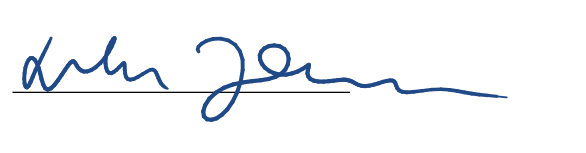
\includegraphics[width=250pt]{signature.png}
\end{document}

















%%